% Deze template is gemaakt door Fons van der Plas (f.vanderplas@student.ru.nl) voor het publiek domein en mag gebruikt worden **zonder vermelding van zijn naam**.
% This template was created by Fons van der Plas (f.vanderplas@student.ru.nl) for the public domain, and may be used **without attribution**.
\documentclass{report}
\usepackage[utf8]{inputenc}     % for éô
\usepackage[english]{babel}     % for proper word breaking at line ends
\usepackage[a4paper, left=1.5in, right=1.5in, top=1.5in, bottom=1.5in]{geometry}
                                % for page size and margin settings
\usepackage{graphicx}           % for ?
\usepackage{amsmath,amssymb}    % for better equations
\usepackage{amsthm}             % for better theorem styles
\usepackage{mathtools}          % for greek math symbol formatting
\usepackage{enumitem}           % for control of 'enumerate' numbering
\usepackage{listings}           % for control of 'itemize' spacing
\usepackage{todonotes}          % for clear TODO notes
\usepackage{hyperref}           % page numbers and '\ref's become clickable
\usepackage{todonotes}
\usepackage{float}
\usepackage{caption}

%%%%%%%%%%%%%%%%%%%%%%%%%%%%%%%%
%% SET TITLE PAGE VALUES HERE %%
%%%%%%%%%%%%%%%%%%%%%%%%%%%%%%%%
%             ||               %
%             ||               %
%             \/               %

\def\thesistitle{Entity Linking in Funding Domain}
\def\thesissubtitle{Thesis Subtitle}
\def\thesisauthorfirst{Gizem}
\def\thesisauthorsecond{Aydin}
\def\thesissupervisorfirst{Dr. Faegheh}
\def\thesissupervisorsecond{Hasibi}
\def\extthesissupervisorfirst{Dr. S. Amin}
\def\extthesissupervisorsecond{Tabatabaei}
\def\thesissecondreaderfirst{name}
\def\thesissecondreadersecond{Surname}
\def\thesisdate{June 2021}


%             /\               %
%             ||               %
%             ||               %
%%%%%%%%%%%%%%%%%%%%%%%%%%%%%%%%
%% SET TITLE PAGE VALUES HERE %%
%%%%%%%%%%%%%%%%%%%%%%%%%%%%%%%%


%% FOR PDF METADATA
\title{\thesistitle}
\author{\thesisauthorfirst\space\thesisauthorsecond}
\date{\thesisdate}

%% TODO PACKAGE
\newcommand{\towrite}[1]{\todo[inline,color=yellow!10]{TO WRITE: #1}}

%% THEOREM STYLES
\newtheorem{theorem}{Theorem}[section]
\newtheorem{corollary}{Corollary}[theorem]
\newtheorem{lemma}[theorem]{Lemma}
\newtheorem{proposition}[theorem]{Proposition}

\theoremstyle{definition}
\newtheorem{definition}[theorem]{Definition}

\theoremstyle{remark}
\newtheorem*{remark}{Remark}


%% MATH OPERATORS
\DeclareMathOperator{\supersine}{supersin}
\DeclareMathOperator{\supercosine}{supercos}

%%%%%%%%%%%%%%%%%%%%%%%

\begin{document}
\begin{titlepage}
	\thispagestyle{empty}
	\newcommand{\HRule}{\rule{\linewidth}{0.5mm}}
	\center
	\textsc{\Large Radboud University Nijmegen}\\[.7cm]
	
\includegraphics[width=25mm]{img/in_dei_nomine_feliciter.eps}\\[.5cm]
	\textsc{Faculty of Science}\\[0.5cm]
	
	\HRule \\[0.4cm]
	{ \huge \bfseries \thesistitle}\\[0.1cm]
	%\textsc{\thesissubtitle}\\
	\HRule \\[.5cm]
	\textsc{\large Thesis MSc Computing Science}\\[.5cm]
	
	\begin{minipage}{0.4\textwidth}
	\begin{flushleft} \large
	\emph{Author:}\\
	\thesisauthorfirst\space \textsc{\thesisauthorsecond}
	\end{flushleft}
	\end{minipage}
	~
	\begin{minipage}{0.4\textwidth}
	\begin{flushright} \large
	\emph{Supervisor:} \\
	\thesissupervisorfirst\space \textsc{\thesissupervisorsecond} \\[1em]
	\emph{External Supervisor:} \\
	\extthesissupervisorfirst\space \textsc{\extthesissupervisorsecond} \\[1em]
	\emph{Second reader:} \\
	\thesissecondreaderfirst\space \textsc{\thesissecondreadersecond}
	\end{flushright}
	\end{minipage}\\[4cm]
	\vfill
	{\large \thesisdate}\\
	\clearpage
\end{titlepage}




\begin{abstract}
Automatic extraction of funding information from academic articles adds significant value to the research community, such as enabling organizations to track the outcome of the research they funded and aiding open access rules. An important part of funding information extraction is detecting mentions of grant numbers and funding organizations, while disambiguating the latter to a knowledge base. For this purpose, various approaches have been proposed. In this thesis, latest general-purpose neural architectures for Named Entity Recognition and Disambiguation are investigated and adapted to the problem of Entity Linking in funding domain. Furthermore, a BERT neural language model is pretrained further with sentences that contain funding information and is used in the proposed neural solutions. The developed approaches are compared with feature-based models, showing a similar performance on disambiguation and a great improvement on mention detection. At the end, precision, recall and F1 scores of 72.5, 78.5 and 75.4 are reached for Entity Linking for funding organizations, and scores of 94, 96.6 and 95.2 for grant mention detection using the developed neural approaches. 
\end{abstract}



\tableofcontents


\chapter{Introduction}
\label{sec:intro}
\section{Background and Motivation}
Automatic extraction of funding information from academic articles has been an interesting subject for researchers, and various approaches have been proposed for this purpose \cite{ElsPaper,AckExtract,GrantExtractor}. Annotating articles with their corresponding funding information adds significant value to the research community. Furthermore, it is not possible to do this annotation manually due to the immense amount of literature, making automatization a must.

A lot of research is made possible by the funding that was provided. Many researchers spend a significant amount of time to find the financial resources they need, and many organizations spend large amounts of capital to sponsor research. This puts funding in an important position for research output, researchers and organizations. As a consequence, displaying funding information of academic articles brings certain benefits. For example, it enables organizations to track the outcome of the research they funded \cite{ElsPaper}. Successful research output on one topic may persuade an organization to invest more in that topic, expanding the resources available to the researches interested in that area. Or, if a researcher is looking for funding for a certain research question, they can search for organizations that funded a similar topic in the past. Lastly, some funding organizations, such as NWO\footnote{\url{https://www.nwo.nl/en/open-access-publishing}} and National Institutes of Health\footnote{\url{https://en.wikipedia.org/wiki/NIH_Public_Access_Policy}},  may require the researchers to make the resulting publications publicly available. Displaying funding information may aid the compliance of such open access rules \cite{GrantExtractor}. 

Funding information extraction contains subtasks in itself. These can roughly be summarized as:\vspace{0.2cm}
\renewcommand{\labelenumi}{(\roman{enumi})}
\begin{enumerate}
     \vspace{-0.3cm}\item isolating the piece of text that contains the funding information from the articles,
     \vspace{-0.6cm}\item extracting the strings that refer to funding organizations and grant numbers from the selected text,
     \vspace{-0.3cm}\item for the strings of funding organizations, determining which real-world organization is being referred to,
     \vspace{-0.3cm}\item for the strings of grant numbers, determining which funding organization string they are related to.
\end{enumerate}

\vspace{-0.3cm}\noindent In this thesis, the aim is to develop a neural Entity Linker for funding domain, hence tackling subtasks (ii) and (iii). 

Entity Linking (EL) is the task of annotating text with corresponding entity identifiers from a knowledge base (KB) \cite{balog}. A KB is a collection of entities representing uniquely identifiable artefacts in real world. An entity could be many things, such as a person, a place or even an artwork. EL entails two subtasks: Named Entity Recognition (NER) and Named Entity Disambiguation (ED). NER corresponds to detecting mentions and their respective types from the text, and ED corresponds to finding which entity in the KB a mention is referring to \cite{balog}. In this definition, mentions are strings in text indicating entities.

A large amount of literature addresses EL, NER and ED using neural approaches, which includes the state-of-the-art methods \cite{REL,LUKE,mulang} as well. These methods show significant improvement over rule-based systems or systems utilizing classical Machine Learning algorithms, such as DBPedia Spotlight \cite{dbpediaspotlight}. The bigger part of the work on neural NER, ED and EL focuses on performing these tasks in general-domain, often times considering Wikipedia pages as entities \cite{nlpnotes}. There is no guarantee that these approaches will perform well in funding domain as there are significant differences. For example, in order to disambiguate funding organizations, a different KB is needed due to most of the smaller funders not being present in general-purpose KBs. Moreover, mentions of organizations that are not funders should not be extracted. In addition, grant numbers are mostly a combination of digits and letters, different from mentions of more popular entities such as persons or places. Another challenge is the limited amount of labelled data. In general-domain setting, Wikipedia could be exploited to extract millions of samples \cite{bunescu-pasca-2006-using}. Supervised neural architectures for NER require a large amount of training data to obtain high performance \cite{NERsurvey}. 

\section{Objective}

The objective of this research is to adapt the current advancements on EL and its subtasks to be able to improve the quality of funding information extraction. Considering the challenges funding domain adds to EL, this thesis aims to answer the following research question:

\begin{quote}\emph{RQ: Is it possible to use neural approaches for Entity Linking in funding domain, where labelled data is limited and a domain-specific knowledge base is used?}\end{quote}

\noindent To be able to answer the main research question, these sub-questions have to be answered first:

\begin{quote}\emph{Q1: How to detect mentions of funding organizations and grants?}\end{quote}
\begin{quote}\emph{Q2: How are the entities going to be represented?}\end{quote}
\begin{quote}\emph{Q3: How will disambiguation be performed?}\end{quote}


\section{Approach and Contributions}
Initially, the literature on general-domain NER, ED and EL solutions is reviewed. Among the reviewed solutions, some of them are selected for experimentation based on specific criteria. It was checked whether the selected solutions perform well compared to others, and whether they can be adapted to the task at hand without losing their core properties. For example, a solution that is based on graph structures was not found convenient, as that information is not available. Moreover, it was valued that the model should offer enough flexibility so that some components can be modified to capture the important aspects of funding information extraction. In addition, it was taken into consideration that the selected solutions should not require too much computational power or too much labelled data as both resources are limited. The literature on domain-specific approaches were also reviewed to obtain some insights on the challenges other domains had faced and the respective solutions. Lastly, various techniques on domain adaptation of neural language models and different entity embeddings were investigated as both emerged to be crucial elements of possible solutions.  

After careful consideration, it was decided to develop two separate components for NER and ED to perform EL instead of a single end-to-end component. This decision was made to have a more explainable system and to have a system that is less computationally demanding to train. For the NER component, two systems are selected: the NER model that is proposed by Akbik et al. \cite{flairlib} and the NER system described in \cite{BERT}, due to BERT's \cite{BERT} recent success. For ED, BLINK's architecture \cite{scalablezeroshot} is selected because of its flexibility and success in zero-shot setting. Moreover, recently an end-to-end neural system to perform EL on questions, ELQ \cite{elq}, is proposed. The architecture of ELQ encompasses the neural candidate selector of BLINK. Hence, it will be possible to extend an ED system built inspired by BLINK to perform mention detection following ELQ. Furthermore, as BERT takes part in the majority of experiments, a BERT model is further pretrained on the funding information sentences and used in both NER and ED systems. 

Elsevier B.V.\footnote{\url{https://www.elsevier.com/}} uses Natural Language Processing (NLP) solutions to extract funding information from academic articles. Later on, this information is displayed in some of its products such as Scopus\footnote{\url{https://www.scopus.com/}}, one of the world's largest citation and abstract databases. Elsevier has a high-quality labelled dataset for this task and a domain-specific KB for funding organizations. The chosen models are trained and evaluated using the labeled dataset provided by Elsevier, and also disambiguation is performed to the provided KB. The developed models are compared with each other and feature-based models to determine the best method and to show the effectiveness of neural approaches.

The contributions of this thesis can be summarized as:
\renewcommand{\labelenumi}{\arabic{enumi}.} 
\begin{enumerate}
    \item Training a new BERT model, BERT$_{SC}$, for funding information extraction and showing its effectiveness.
    \item Developing a neural EL solution to extract mentions of funding organizations and grant numbers simultaneously, and to disambiguate the former to a domain-specific KB. 
    \item Modifying BLINK's candidate selection architecture to makes use of a binary classification setting for reducing the amount of memory required during training and for incorporating NIL mentions intuitively.
    \item Showing the effectiveness of a minimal linear reranker that can work with the proposed candidate selector.
\end{enumerate}

We believe that this research will be influential for other domains to make use of the state-of-the-art neural architectures for EL and will provide important insights on possible strengths and weaknesses of utilizing such systems. Moreover, the developed neural components could be used as a part of a single end-to-end funding information extraction model in the future. The code for the developed models can be found on GitHub\footnote{\url{https://github.com/gizemayydin/Entity-Linking-in-Funding-Domain}}.

\section{Outline}
The aim of Chapter \ref{chap:rw} is to review the recent literature on NER, ED and EL, as well as various domain-specific solutions to these problems. Literature on entity embeddings and domain adaptation of neural language models are also touched upon due to their relevance in proposed solutions. Lastly, notable previous work on funding information extraction is presented. In Chapter \ref{chapter:Approach}, the task of EL in funding domain is formally defined, the approach to tackle this task is presented and the models used are explained in detail. The dataset used, experimentation, results and discussion is included in Chapter \ref{sec:Evaluation}. Chapter \ref{chapter:Conclusion} concludes this thesis by summarizing the findings and providing a course of direction for future research.

\chapter{Related Work}
\label{chap:rw}
%\cite{BERTLayers}: they also report fine tuning is end to end instead of feature based approach even when all labels are combined (check conclusion)
There is a large amount of literature on Entity Linking (EL) and its subtasks, Named Entity Recognition (NER) and Entity Disambiguation (ED). The bigger part of this literature focuses on performing these tasks in the general-domain setting, often times considering Wikipedia pages as entities \cite{nlpnotes}. While this line of research introduces the state-of-the-art approaches, there is no guarantee that these approaches will perform well in a domain-specific setting with a custom knowledge base (KB). Hence, domain-specific literature is also investigated to get insights on adapting general-purpose methods to specific domains.

Section \ref{FundingDataExtraction} reviews the literature on automatic funding information extraction from academic articles. In Sections \ref{sota1}, \ref{sota2} and \ref{sota3} state-of-the-art general-purpose NER, ED and EL solutions are presented. Domain-specific neural NER, ED and EL approaches are demonstrated in Section \ref{domSpec}. Section \ref{entityRep} concentrates on entity representations in neural ED, mainly entity embeddings, and lastly, Section \ref{preLMDiffDomain} reviews the literature on domain-adaptation of neural language models.

\section{Funding Information Extraction}
\label{FundingDataExtraction}

    One of the most notable work on automatically extracting funding information from text is FundingFinder \cite{ElsPaper}. FundingFinder is a two-step pipeline that utilizes NLP techniques. In the first step, the paragraphs that contain funding information are determined, and in the second step, NER is performed using an ensemble of different Sequential Learning approaches. The authors also created a publicly available benchmark dataset for this task. The approach used in this thesis builds upon this work, keeping the first step intact while improving the second step, and adding the ED capability. 
    
    Before FundingFinder, not much literature existed on extracting funding information from text automatically, and the existing work mostly utilized regular expressions \cite{ElsPaper}. Recently, there have been more approaches presented to tackle this problem. In 2020, Wu et al. proposed AckExtract  \cite{AckExtract}, which extracts funder organization mentions from the COVID-19 Open Research Dataset \cite{CORD}. For NER, they use a pretrained neural model from the package Stanza \cite{stanza}, which uses Contextual String Embeddings \cite{flairpaper}. However, their method does not include any ED, whereas in this thesis, one of the tasks is to link the funder mentions to their corresponding entities in the domain-specific KB. Another approach is proposed in 2021, GrantExtractor \cite{GrantExtractor}, which extracts funding information from articles in biomedical literature, in the form of grant numbers and their corresponding organizations. For extracting grant numbers, they train a BiLSTM-CRF \cite{BiLSTMCRF} architecture. Using a multi-class classifier, they determine which organization the extracted grant number belongs to. They do not use any neural approaches for extracting organization mentions. Also, the focus of GrantExtractor is on linking grant numbers to their respective organizations, while the focus of this thesis includes extracting all funding organizations that financially supported the corresponding research, even though no grant information is acknowledged.

\section{Named Entity Recognition}
\label{sota1}
In the past couple of years, Deep Learning has been a popular choice to tackle the NER problem, and the corresponding research has improved the state-of-the-art results \cite{NERsurvey}. In 2018, Akbik et al. proposed Contextual String Embeddings \cite{flairpaper}, which represents words using a character-level neural language model, and is able to produce different word embeddings depending on the context. By utilizing a BiLSTM-CRF architecture that takes the concatenation of Contextual String Embeddings and pretrained GloVe embeddings \cite{glove} as input, they report state-of-the-art results in both German and English NER, in the CoNLL-2003 \cite{conll} setup. In 2019, Devlin et al. introduced BERT \cite{BERT} which obtained new state-of-the-art results on several tasks. In English CoNLL-2003, they obtained an F1 score of $92.8\%$ using the cased version of BERT$_{BASE}$ \cite{BERT}, performing very close to \cite{flairpaper}, which obtained $93.1\%$. It is believed that both of these models could be suitable for extracting mentions of funding organizations and grant numbers, as they do not necessarily require extensive amount of labeled data and there is no dependency to any resource that is not available.

Some approaches for NER utilize external resources, such as a list of entity names, which may be called a dictionary or a gazetteer. This may boost the performance of the system, but may also hurt the generalization ability \cite{NERsurvey}. However, there have been various models presented \cite{NERgazetteer, NERDict} that incorporate this information while performing comparable to \cite{flairpaper}. With this approach, both papers \cite{NERgazetteer, NERDict} aim to improve the performance on entities that do not appear in the training set or that are rare. These features may also be useful for this work, as the domain-specific KB contains various synonyms for each funding organization, and most of the entities available do not appear in the dataset (see Section \ref{sec:EvalExpSetupData}).

Recently, Yamada et al. (2020) proposed LUKE \cite{LUKE}, a contextualized representation for both words and entities, to be used in entity-related tasks. LUKE is based on the bidirectional transformer \cite{transformer}, however, it treats words and entities as independent tokens. For this purpose, the authors propose a modified attention mechanism as well as a new training methodology based on BERT's masked training. They pretrain LUKE using a large entity-annotated Wikipedia corpus. By using the proposed embeddings, they report the new state-of-the-art results for NER, improving upon \cite{flairpaper}. The entities that are included in this work differ significantly from the ones that are in Wikipedia or in any other famous general-purpose KB. Hence, we do not expect to obtain any gain from using LUKE instead of an NER component based on BERT$_{BASE}$ or the one introduced by \cite{flairpaper}.

\section{Entity Disambiguation}
\label{sota2}

One of the most influential work in ED is MentNorm \cite{mentnorm}, proposed by Le and Titov in 2018. MentNorm is a multi-relational neural model, and is based on the assumption that the relations between co-occurring entities provide important clues for disambiguation. Different from preceding work, they model these relations as latent variables, which enable to learn these in a way that is most useful for the ED task. They report a micro averaged F1 score of 93.07\% on AIDA-B CoNLL YAGO dataset \cite{CoNLLYago}, outperforming previous research. Despite being successful, collective ED methods may suffer from high complexity \cite{dca}. In 2019, Yang et al. \cite{dca} proposed Dynamic Context Augmentation (DCA) that can perform collective ED with just a single pass over the whole document. DCA takes global entity coherence into account, but instead of processing the whole document at once, it processes each mention sequentially. The authors reason that this methodology is more intuitive as humans have the ability to make inference while reading, without having read the whole document. The information of previous linked entities are accumulated and used for disambiguating the proceeding mentions. Their best configuration 94.64\% accuracy on AIDA-B CoNLL YAGO dataset, which is higher than that of \cite{mentnorm}. In funding domain, the number of Organization mentions per document is much less than that of public benchmark datasets. For example, \cite{dca} report an average of 19.4 mentions per document for AIDA-B dataset. In the dataset for funding information extraction, this number is around 3. Moreover, entity co-occurrences do not provide important clues for disambiguation. That is why collective ED systems are not used for this work.

In 2018, Raiman and Raiman proposed DeepType \cite{raiman} for ED, a neural network that is constrained by the predicted type information for a given entity. By using the type information, they also reduce the complexity of disambiguation from polynomial to linear. DeepType produced state-of-the-art results in three ED datasets, by obtaining scores of 92.36\%, 94.88\% and 90.85\% on WikiDisamb30 \cite{wikidisamb}, CoNLL (YAGO) \cite{CoNLLYago} and TAC-KBP-2010\footnote{\url{https://tac.nist.gov/}} respectively. The authors also note that DeepType can reach 99.0\% and 98.6\% accuracy on CoNLL (YAGO) and TAC-KBP-2010, when the type information is provided by an Oracle. Based on that, they claim the ED problem can almost be solved if the type classifier is improved. However, in the case of funding domain, most of the ambiguities in mentions cannot be solved by using the type information. For example, the mention ``Ministry of Health'', can be resolved to different entities corresponding to ministries in different countries, however,  the types of these entities would be the same.

The paper proposed by Mulang' et al. (2020) \cite{mulang} slightly advances the state-of-the-art ED results for CoNLL (YAGO) dataset by obtaining a score of 94.94\%. The authors introduce the idea of incorporating context derived from Knowledge Graphs (KG) to pretrained transformers with the aim of improving their performance for ED. They extract triplets from the KG, verbalize them into natural language form, and append them to the input sentence and mention before passing it through the transformer. When they replace the Wikipedia description used in the DCA-SL model \cite{dca} with the structured KG context they extracted, they obtain the above-mentioned score. In this work, there is not a KG that could be utilized in such manner. Otherwise, incorporation of the work by \cite{mulang} could have added value to the current system.

Another interesting approach for ED is DEER \cite{googleintern},  proposed by Gillick et al. in 2019. The model is essentially a dual-encoder, one to encode the mention and its context, and another to encode the entity using its description and categories. Then, the model is trained to maximize the cosine similarity between the encoded representations of the correct mention - entity pairs. The authors use hard negatives during training, and they show the positive effect of this to the performance.  As the second encoder utilizes only entity information, entity embeddings can be precomputed beforehand, and hence only one encoder is run during inference. We believe that this work can be very influential for this thesis. They show good performance on public benchmark datasets, the inference time is fast even though it is a neural approach, and can scale up to unseen entities. The only downside is that each encoder has sub-architectures within itself. For example, the entity encoder has three different encoders for the title, the category and the first paragraph of the description. Hence, it may be hard to adapt these for the information available.

Wu et al. (2020) \cite{scalablezeroshot} proposed BLINK, which outperforms DeepType \cite{raiman} in TAC-KBP-2010 by obtaining a 94.5\% accuracy . Their method also achieves state-of-the-art results in the zero-shot Entity Linking dataset derived from WikilinksNED \cite{wikilinksned}. To perform ED, they only use textual information, and architectures that utilize pretrained BERT transformers. They represent the mention using itself and its context, and the entity using its description. Using a biencoder \cite{polyencoders}, they encode the mention and entity representations in the same space, which they later use to extract candidates for a given mention using approximate nearest neighbor search. To train the biencoder, they make use of a hard negative mining strategy inspired by \cite{googleintern}. They make the final decision by passing representations of the candidate entities and mentions through a cross-encoder \cite{polyencoders}. BLINK can perform well for unseen entities and has an architecture that is easy to adapt to the problem at hand. Hence, BLINK is found highly suitable for this work, and is investigated further (See Section \ref{sec:entdismethod}). 

Even though there had been many influential work on tackling ED, not many of them encompass NIL mentions, mostly excluding them from evaluation. In this work, NIL mentions mostly refer to emerging entities, and hold high importance. New organizations are being added frequently, and NIL mentions give important insights on these organizations. They are also used to refine the KB from time to time. One of the hardest cases of NIL mentions occurs when the emerging entities have ambiguous names \cite{NILMentions}. These cases also exist in the funding domain. For example, ``Ministry of Education'' could refer to different organizations based on the country, and it could be that the ministry of a country is not in the KB. Then, the ED system should infer that this mention does not refer to any other ministries that are included in the KB. Moreover, there are organizations that share the same acronym as a coincidence. It could be that a funder that does not exist in the KB is acknowledged by using its acronym, which matches a completely different organization that happens to be in the KB. Hoffart et al. (2014) \cite{NILMentions} proposes a novel method to detect such emerging entities. They add an additional instance representing an emerging entity to the candidate set of each mention. They initially model this instance using the string of the mention, but then enhance the representation based on keyphrases utilizing latest news streams. This is not applicable for this research as ED is performed on academic articles. They also define confidence scores based on perturbing mentions and entity decisions around the input mention. However, in this work, the models investigated do not make use of collective disambiguation.

\section{Entity Linking}
\label{sota3}

Kolitsas et al. (2018) \cite{kolitsas} proposed the first end-to-end neural EL system in 2018, and recorded state-of-the-art results in AIDA CoNLL dataset. By tackling NER and ED jointly, the authors aim to utilize the dependency between these two tasks. They suggest that this has several benefits, such as improved mention boundary recognition. Their method first extracts all possible mention spans from the input. Then, the model computes a score for each mention - candidate entity pair, using pretrained entity embeddings \cite{kolitsasEmbed}, context-aware mention representations, commonness and long range attention scores. The final output for the input text is based on these scores and global entity coherence. This approach has some properties that make it not suitable for this thesis. First, the entity embeddings they use are for Wikipedia entities, thus new embeddings for this KB must be obtained beforehand somehow. Based on the properties of these new embeddings, the global coherence layer should be reconsidered. Also, the runtime could be a problem as the methodology involves extracting all possible mention spans. As the grant mentions do not go through ED, the loss needs to be adapted accordingly. Lastly, the advantage of this approach is that the mention boundary detection is improved by combining NER and ED, which is shown by the fact that there is only a small difference between the weak and strict matching evaluations. However, the authors report that most of their mentions consist of at most two words, which is not true for funding organizations that tend to have longer names. Hence, there is no guarantee that this advantage will persist in funding domain.

Another neural approach that can perform both NER and ED in an end-to-end fashion is proposed by Martins et al. in 2019 \cite{StackLSTM}. The approach makes use of Stack-LSTMs \cite{actualStackLSTM} to detect mentions on the fly rather than detecting them for the whole sequence at a time. For each token in the sequence, an action is predicted. This action can be: \textit{Shift}, \textit{Out} or \textit{Reduce}.  \textit{Out} means that the token at hand is not part of a mention, while \textit{Shift} means that it is.  After all the tokens of the mention is marked with consecutive \textit{Shift} operations, \textit{Reduce} is performed, meaning that the detected mention is disambiguated. There are multiple \textit{Reduce} actions, one for each mention type. Hence, the type of the \textit{Reduce} action also predicts the type of the mention. The model outputs a probability distribution over the possible action space for each step, and the action with the highest probability is selected. In the disambiguation step, first, the mention is classified to determine if it is a NIL-mention or not. If it is not, a candidate entity set is selected with respect to entity embeddings obtained by \cite{yamada-etal-2017-learning} and prior probabilities. Then, a score is assigned to each candidate entity by utilizing an affine transformation function, and the mention is linked to the entity with the highest score. The model is trained with a multi-task learning setting of three tasks: NER, NIL-mention detection and ED. For NER, the loss is calculated as the cross-entropy between the gold actions and the selected actions. For NIL detection, binary cross-entropy is utilized. Lastly, for ED, cross-entropy over the candidate entities is calculated. The authors show that performing NER and ED jointly benefits both of the tasks, by comparing the performance of a joint architecture with two different architectures. However, for the NER task, both \cite{flairpaper} and \cite{BERT} outperform the work of \cite{StackLSTM}, and in terms of EL, the work fails to outperform \cite{kolitsas}. This work is still very influential, especially as they include NIL-mentions in their research.

In 2020, van Hulst et al. proposed REL \cite{REL}, an EL toolkit that utilizes state-of-the-art NLP research, outperforming \cite{kolitsas} in terms of micro F1 score in AIDA CoNLL dataset. REL tackles the EL problem in three steps: NER, candidate selection and ED. For NER, they utilize Flair, namely, the sequence labelling architecture and Contextual String Embeddings proposed by \cite{flairpaper}. For each mention, up to 4 candidates are selected using commonness, and up to 3 candidates are selected based on the similarity between the context of the mention and entity embeddings. Entity embeddings are provided by \cite{kolitsasEmbed}, the same ones used in \cite{kolitsas}. For ED, MentNorm by Le and Titov \cite{mentnorm} is used. Apart from obtaining state-of-the-art results, REL also offers a modular architecture, allowing easy replacement of components and it does not require a GPU during inference time \cite{REL}. The success of REL in terms of performance and efficiency is one of the factors why Contextual String Embeddings are in the agenda of experiments for this work. However, MentNorm is not suitable for funding domain because of its dependency on entity coherence. This work also inspired this research in the sense that a comparable or higher performance than that of \cite{kolitsas} can be obtained even when NER and ED are performed separately, which is advantageous in terms of runtime and explainability.

Broscheit (2020) \cite{bertEL} proposed an architecture that jointly does NER and ED using BERT. In this approach, the task of EL is framed as a per-token multi-class classification problem. The model utilizes a pretrained BERT model and an output classification layer on top of it. Even though this approach is a big simplification on the EL task, it performs only a few points off compared to \cite{kolitsas}.  However, as each entity is cast as a class, the model cannot disambiguate unseen entities. In real-word, KBs keep growing, and hence it is important for the system to be extendable for entities that do not exist in the training set \cite{gupta}. Moreover, some training datasets may not cover the whole entity vocabulary, such as the one used in this work. However, this research is very inspiring in terms of showing BERT's capability to learn the task of EL. It also contributed in the decision process of experimenting with BERT as a neural language model to be used in this work.

In 2021, De Cao et al. proposed GENRE \cite{GENRE}, a novel approach for end-to-end EL. The authors criticize previous work on various aspects, such as the need of hard negatives during training and the use of dot product to model the relevancy between an entity and a mention. GENRE addresses these shortcomings by using a sequence-to-sequence generative architecture for EL. For this purpose, the authors fine-tune a BART \cite{bart} model on the task. Mention detection and disambiguation is achieved by decoding the input sequence which is done dynamically. For each step in sequence generation, the model has various options: generate a mention span, generate a link for the mention or continue copying the input sequence. To start generating a mention, the model has to generate a mention-start-tag. Inside the mention, the model can either copy the input sequence or stop mention generation by generating a mention-end-tag. The latter puts the model in the link generation (i.e. disambiguation) state. In GENRE's architecture, each entity is associated with a unique textual identifier, such as a name. The model assigns a score to each entity based on the generative probability of the corresponding entity's name given the context. As the entity space is large, a Beam Search \cite{beamsearch} variant (Constrained Beam Search) is used. This whole schema allows the model to generate an output sequence with detected mentions and their corresponding entities, while narrowing the possible search space. The authors report that there is no need for hard negative mining, as the loss for training is based on maximizing the likelihood of the output sequence, and can be calculated exactly \cite{GENRE}. Lastly, the model has a much smaller memory footprint compared to previous approaches as it does not need to store precomputed entity embeddings, and either outperforms or performs on par with the state-of-the-art for various public benchmark datasets. Even though GENRE has an outstanding performance, there are various concerns on using it for funding domain. The authors report that large generative models benefit from more data, and hence they pretrain their model with a large amount of labeled data. This is not possible for this work as there is no such dataset available. Moreover, the entity representation is based on having a unique string such as a name for each entity. In funding domain, organizations may have more than one official name such as acronyms or names in other languages, or there may be different organizations with the same name. To create a unique name per organization, some of these alternative names should be concatenated, and it is not clear whether this kind of representation would work with GENRE, or whether it would be tractable given that the inference is dependent of the size of entity representation. Moreover, the authors report that their entity representations had 6 tokens on average for the experiments, which is not realistic for funding organizations.

\subsubsection{Entity Linking in Queries}
There is a specific line of work that focuses on EL in queries and questions. Questions differ from well-formed sentences, and tend to be shorter and noisier, hence bring additional challenges \cite{elq}. In addition, the context is much more limited \cite{ELinConv}. The input for funding information extraction is not as long as a document, and is also not as short as a query. Hence, this makes both lines of work interesting for this thesis.

Zi et al. (2020) \cite{elq} proposed ELQ, an end-to-end EL system for questions. ELQ extends BLINK's biencoder by adding the mention detection capability to the model. The resulting model outperforms the state-of-the-art in two benchmark Question Answering datasets in terms of EL capabilities. The end-to-end architecture of ELQ differs significantly from that of \cite{kolitsas}, improving the efficiency and bringing some flexibility. Even though all possible mention spans are extracted from the text for mention detection, different from \cite{kolitsas}, the spans are thresholded based on some probability and length. This eliminates the need to run a candidate selector to limit the mention space. In their experiments, the authors set the maximum span length to 10, which is still not optimal for organizations but is not unrealistic. Also, they jointly optimize the NER and ED losses, which may allow to extend the system for Grant mentions. Another advantage is that they do not need to train the entity encoder as they obtain it from BLINK. Even though the entity encoder of BLINK is for Wikipedia entities, it is possible to get embeddings for other KBs by adjusting the entity representation and retraining the model. Despite this system being for questions and thus being evaluated on data with a significantly different distribution, it is worth to inspect its performance for the task at hand, as the authors show optimism towards ELQ's performance on longer and structured documents.

\section{Domain-Specific Systems}
\label{domSpec}
In this section, the research that aims to tackle EL, NER and ED in a domain-specific setting with neural architectures is reviewed.

For NER, there is a great amount of research in general domain, however, more research on domain-specific solutions is expected for supporting real-world applications \cite{quote1}. Existing NER approaches rely on a large amount of annotated data, which may not be available for the domain-specific setting \cite{NERDict2}. Hence, Shang et al. (2018) \cite{NERDict2} proposed AutoNER, a neural architecture that is designed to learn from data that is created by distant supervision, without any human effort. AutoNER uses domain-specific dictionaries to automatically generate labelled data with distant supervision. The authors also introduce the ``Tie or Break'' tagging schema, that is based on predicting whether two adjacent tokens belong to the same mention or not. They reason that this tagging scheme is suitable to use noisy labels generated by distant supervision. They show the effectiveness of their work in multiple datasets, two of them being the BC5CDR \cite{bc5cdr} and NCBI-Disease \cite{ncbi} datasets from the biomedical domain, in which AutoNER achieves 84.8\% and 75.52\% F1 score respectively. For this work, as there is already labeled data available, it is believed that such labeled data generation should be used only if the high quality data at hand proves to be insufficient significantly.

Another domain-specific NER approach that utilizes a dictionary is proposed by Wang et al. (2019) \cite{MedDict}, which tackles the Clinical NER problem in Chinese text. They show the effect of incorporating dictionary knowledge in the BiLSTM-CRF architecture on rare and unseen entities experimentally. Also, they suggest five different methods of using dictionaries in this context and compare the results. This work can be very influential for funding domain, as a large dictionary is available, and the proposed features can be incorporated to any neural architecture easily, enabling to utilize both this resource and the labeled data.

There also exist research on tackling the domain-specific ED problem with neural architectures. In 2019, Mondal et al. \cite{MedicalTriplet} proposed a system that is based on string similarity to perform ED on disease names. The authors utilize a two-step solution. First, for each mention, they extract a set of candidate entities based on Jaccard overlap and the cosine similarity between the entity label and the mention. They use word embeddings to calculate the cosine similarity. For multi-word strings, they sum the embeddings for each word. Then, they rank the candidate entities with a Triplet Network \cite{tripletNetwork}, that learns to reduce the distance of the mention with the positive candidate, while increasing the distance with the negative candidate. As an input to this network, word embeddings is used again to represent the mention and the candidate entity's label. With this approach, they obtain 90\% accuracy on the NCBI-Disease dataset, outperforming previous approaches. The drawback of this approach is that it does not utilize any context information, which is important for funding domain, because clues such as the country of the organization can be found in the context. Moreover, multi-word mentions are very common for organizations, and summing the embeddings may not be the best way to incorporate each word to the representation.

The input representation of entities vary between different approaches. In another research tackling clinical ED by Schumacher et al. (2020) \cite{ClinicalConcept}, different from \cite{MedicalTriplet},  multi-word strings are represented by two different methodologies, Max Pooling over the word embeddings and running self-attention. The authors report that running self-attention produces better results compared to Max Pooling. The proposed methodology also addresses some issues that come with funding domain, such as the importance of the lexical similarity between the mention and an entity. Moreover, the architecture resembles the Biencoder of BLINK in terms of having two components to encode the mention and entity. However, in this work, ELMO \cite{elmo} is used and the encoders have shared parameters. Also, the loss and negative mining strategy is different. The success of this work is inspiring in terms of showing that it is possible to use such a dual architecture for domain-specific problems. 

Using BERT instead of ELMO could have some benefits for entity representation, for example, the [CLS] token can be used to represent the whole sequence naturally. For example, Sung et al. (2020) \cite{sung-etal} represents each mention and each synonym of an entity using BERT's [CLS] token for the biomedical domain. On top of that, another representation based on TF-IDF scores is also introduced. For disambiguation, the authors define two different similarity function for each of these representations. The final similarity of a mention and an entity synonym is defined based on the weighted average of these two similarity scores. It is believed that utilizing such a sparse representation could possibly add value in the funding domain as well. However, this will not be experimented with as it is decided that the additive value of it shown by the results of the paper is not significant enough compared to the time that should be spent for the incorporation of such representation. 

Architectures utilizing the type information are also present. Zhu et al. (2020) introduced LATTE \cite{latte}, an architecture for ED in medical domain. The authors emphasize the importance of fine-grained types in their setting, and as this information is not available, they model the fine-grained types as latent variables. For ED, in addition to the latent fine-grained types, they use the similarity between the entity's label, and the mention and its context. To train their model, they use multi-task learning for both type classification and ED. Even though LATTE is a very inspiring research, it would not have the same affect on funding domain as the reliability to the type information for disambiguation is highly limited.

Some proposed methodologies tackle the EL problem as a whole in a domain-specific setting using neural architectures. For biomedical domain, Zhao et al. (2019) \cite{MedFeedback} proposed a joint neural architecture for NER and ED tasks for performing EL. Their architecture utilizes explicit feedback between the two tasks in a multi-task learning setting. With this architecture, they obtain F1 scores of 87.43\% and 88.23\% in NER and ED tasks of the NCBI-Disease dataset respectively, and 87.62\% and 89.17\% in BC5CDR dataset. With these numbers, they outperform AutoNER in NER setting for both datasets, and perform comparable to \cite{MedicalTriplet} in NCBI-Disease dataset for ED. As the task of ED is framed as classification over the controlled entity set, it is not clear whether the model would work in zero shot setting.

Biomedical domain is not the only one in which neural approaches are used for NER, ED and EL. In 2019, Espejo-Garcia et al. \cite{agricultural} proposed a solution to extract named entities that refer to the important parts of phytosanitary regulations, which is related to the agricultural domain. The authors experimented with eight different state-of-the-art neural architectures. For their setting, the best performing architecture was a bidirectional LSTM \cite{bilstm} that utilized a Softmax layer for inference and got the concatenation of pretrained Word2Vec \cite{w2v} embeddings with character based word representations as input. With this architecture, they obtained an F1 Score of 88.3\%. Apart from agricultural domain, Yang et al. (2020) \cite{cosmetic} proposed Headword Oriented Entity Linking, an EL setting where the mention scopes do not need to be identified, to extract cosmetic products from blogs and to disambiguate them to a domain-specific KB. First, using word segmentation techniques, they identify the headwords of the mentions. Then, they apply classification on the mentions to decide whether the mention can be linked to a product that is in the KB. Lastly, they use a modified version of the architecture proposed by \cite{gupta} for ED.  Another interesting study is by Kurz et al. (2020) \cite{TechTickets}, where they experiment with different BERT-based architectures to disambiguate mentions of machine parts and errors belonging to German technical service tickets.

\section{Entity Representation}
\label{entityRep}

In neural ED, entity representation plays an important role. Some research frames the problem as multi-class classification and represent entities as different classes \cite{bertEL,MedDiffArc,MedFeedback}, while other research tends to use architectures that takes properties of entities as input and learns a representation internally during training for ED \cite{scalablezeroshot}, implicitly or explicitly. Another line of research utilizes entity embeddings \cite{REL,kolitsas,dca,MedicalTriplet}. In this section, the literature on entity embeddings will be reviewed.

There is a large body of literature on embedding entities and relations found in KBs. One of the most notable work is TransE \cite{TransE}, introduced in 2013. TransE generates embeddings for each entity and relation in the input KB. The idea behind TransE is to model relations as translations in the embedding space. For a given triplet $(h,l,t)$ in the KB where $h$, $l$ and $t$ denote head entity, relation and tail entity respectively; TransE aims to make the embedding of $t$ as close as possible to the sum of the embeddings of $h$ and $l$, using an energy-based model. Later on, there has been models that improved upon TransE such as TransH, TransR, CTransR and TransD, each improving upon the previously proposed one respectively  \cite{TransEimproved}. Another interesting work that generates entity embeddings utilizing the triplets in KBs is RDF2Vec \cite{RDF2Vec}. RDF2Vec extracts graph sub-structures, and treats them as sentences to train a Word2Vec model. 

Wikipedia2Vec \cite{wikipedia2vec2} is also a famous and successful method for obtaining entity embeddings. Wikipedia2Vec pretrained embeddings are also available for direct use. Wikipedia2Vec encodes words and entities in the same space and utilizes Word2Vec. To train Wikipedia2Vec, they use three models. Word-based skip gram model puts the embeddings of words that occur in similar context close, anchor context model puts the embeddings of entities close to embeddings of words that occur near the anchor texts of the entity, and lastly, link graph model puts the entity embeddings close based on Wikipedia's hyperlink graph. 

Although proven to be very successful, it is not very likely that embeddings such as Wikipedia2Vec or TransE would perform well for funding organizations. These kind of systems rely heavily on KGs and diverse relations between entities. Besides, it would not be possible to use the already-trained ones, due to the fact that the entities at hand not being present in general-purpose KBs. In the domain-specific KB used for this work, although there exist some relations between entities, they are sparse and not informative in terms of disambiguation. Hence, it is believed that other ways of representation is needed to make sure the available information is utilized fully. Some ED architectures such as BLINK and DEER train a dual architecture that encodes entities and mentions separately. This allows learning entity embeddings that are directly relevant with the data and task at hand. Moreover, it is again possible to precompute these embeddings and store them for efficient inference or for using in other tasks. In this work, such architectures are favored because of their success and flexibility on obtaining entity embeddings by being able to utilizing different representations.

The dual architectures are not the only type of ED systems that allow learning entity embeddings with the task. In 2017, Gupta et al. \cite{gupta} proposed a neural architecture that can generate entity embeddings by jointly encoding the information on the entity's description, the context of its mentions and its type. The architecture consists of three models that encode different information. The parameters of the models and the embeddings are jointly learned based on the sum of four different losses that ensure the entity embeddings and the encoded information is similar. The summation guarantees that entity embeddings can be generated even though some information is missing, such as the description \cite{gupta}. They also proposed an ED model based on these embeddings. As mentioned in Section \ref{domSpec}, a modification of this architecture is used to create entity embeddings in \cite{cosmetic}, showing that the model can be utilized for different types of information as well. The downside of this methodology, for example when compared to BLINK, is that new models and losses should be defined and incorporated into the architecture for using different information. In BLINK, it is possible to just modify the input representation of the entity for the same purpose.

\section{Using Pretrained Language Models in Domain-Specific Applications}
\label{preLMDiffDomain}
BERT, and other pretrained language models have been used extensively in various NLP applications and have obtained state-of-the-art results in benchmark tasks \cite{pretrainedLM}. However, for some domains, they may be too generic and may not be able to cover specific needs \cite{quote2}. Hence, it may be worthwhile to adapt the pretrained language model that will be used to the specific domain. Gururangan et al. (2020) \cite{DontStop} shows that a second-round of pretraining of a pretrained language model improves the performance in both low and high resource settings, using different domains and tasks. Also, Fraser et al. (2019) \cite{quote3}, reports that language models which are pretrained with domain-specific text perform better on the task of NER in biomedical domain. However, it should be noted that training a neural language model from scratch for a specific domain can take weeks \cite{tritrain}. 

There is emerging research on domain adaptation of pretrained language models that is not as costly as training them from scratch. Gururangan et al. (2020) \cite{DontStop} proposed Task-Adaptive Pretraining (TAPT), which corresponds to pretraining the neural language models further with the unlabeled data of the task at hand. They report that this approach performs comparable to pretraining with larger amount of text from the same domain. TAPT is intuitive, has a well-documented open-source implementation and does not require additional resources which makes it easy to use. 

Tai et al. (2020) proposed exBERT \cite{exBERT}, a low-cost method to perform domain adaptation and to add new domain-related words to the vocabulary of BERT while not changing its weights. The authors accomplish this by adding an extension module to the embedding layer and to each transformer layer. The authors show the effectiveness of their approach on biomedical domain. In funding domain, even though the input distribution is different, vocabulary changes as substantial as in biomedical domain is not expected. Hence, expanding the vocabulary of the original BERT is not needed. 

Another methodology is introduced by Poerner et al.  in 2020, and is called GreenBioBERT \cite{word2vectoBERT}. GreenBioBERT stands out by not requiring a GPU and hence being environment-friendly. In this approach, a Word2Vec model is trained on the domain-specific data, and the embedding vectors of the pretrained language model is aligned based on that. The authors evaluate their model on Biomedical NER and compare it to BioBERT \cite{biobert}. Even though BioBERT outperforms GreenBioBERT, it shows that it is still possible to perform domain adaptation in a low-resource setting.



\newpage
\chapter{Approach}
\label{chapter:Approach}
To tackle the Entity Linking (EL) problem in funding domain, a two-step solution is developed. The first step is Named Entity Recognition (NER) and the second step is Entity Disambiguation (ED). For both of these steps, after an extensive literature review, state-of-the-art systems that can be adapted to the problem at hand are determined.

For the NER component, several models were implemented and tested. The first model that is tried is the sequence labelling architecture proposed by Akbik et al. in 2018 \cite{flairpaper}. The choice of experimenting with this model was due to its success in English NER. Moreover, this model is used by REL \cite{REL}, a system that achieved state-of-the-art results on EL, and AckExtract \cite{AckExtract}, a system for extracting funder organization mentions. This model will be denoted as Flair$^{NER}$.

Flair$^{NER}$ is based on Contextual String Embeddings (CSE) \cite{flairpaper}, which are obtained using the concatenation of vectors from a Left-to-Right and a Right-to-Left language model. However, \cite{BERT} reports that BERT is inherently more powerful than such language models as it is using MLM objective, that enables it to train a single representation for which both right and left contexts are used. Because of this claim and the recent popularity of BERT models, it is decided to experiment with BERT as well, which will be denoted as BERT$^{NER}$. 

As recent research showed the importance of domain adaptation \cite{DontStop,exBERT,quote3}, a BERT model is pretrained further on funding acknowledgement sentences using Task-Adaptive Pretraining (TAPT) \cite{DontStop}. This model is denoted as BERT$_{SC}$. Later on, an NER model is trained using BERT$_{SC}$, BERT$_{SC}^{NER}$. 

For the ED component, the biencoder of BLINK architecture proposed by Wu et al. (2020) \cite{scalablezeroshot} is implemented. BLINK consists of two models, a biencoder inspired by \cite{polyencoder} for candidate entity selection and a cross-encoder \cite{polyencoder} for candidate entity reranking. As input, it utilizes mentions with their surrounding context and entity titles with their descriptions. The reason why this architecture was chosen is five-fold. First, BLINK can work in zero-shot setting, which is needed for this research as the training data does not cover the whole entity space. Second, the inference time is not long, and third, the authors demonstrate that this approach obtains state-of-the-art performance on both zero-shot and general setting. Lastly, BLINK's architecture can be adapted to the setting of this work without losing any important properties, and it can be extended to perform end-to-end EL following the ELQ architecture \cite{elq}. In this work, for efficient inference, a linear model is used as a reranker instead of the cross-encoder.

Section \ref{sec:taskdef} defines the problem this thesis is tackling formally. Section \ref{sec:BERT} focuses on the BERT architecture and the domain adaptation procedure. Section \ref{sec:NERMEThod} introduces Flair$^{NER}$, BERT$^{NER}$ and BERT$_{SC}^{NER}$, and Section \ref{sec:entdismethod} explains the methodology used for ED.


\section{Formal Task Definition}
\label{sec:taskdef}
Given a piece of text $d=\{x_1,...,x_N\}$ of $N$ tokens, the task of NER is to identify a set of spans $M = \{m_i \mid m_i = \{x_s,..,x_e\}, s \geq 1 \land s\geq e \land N \geq e\}$, where each span corresponds to a mention. Usually, detecting the types of the extracted mentions is also part of the NER task. The available mention types differ among systems based on their objectives. In this thesis, each mention $m_i$ corresponds to either a \textit{Funding Organization} ($ORG$)  or a \textit{Grant Number} ($GRT$). Hence, $type(m_i) \in \{ORG,GRT\}$. Throughout this research, it is assumed that the mentions are not nested and are not overlapping.

Given the set of mentions $M$, the aim of ED is to link each mention to their corresponding entity $e_i \in \mathcal{E} $ in a KB. A knowledge base is a collection of entities, and may contain information on the entities and relations between them. The contents and specifications of the KB used is task-dependent. The task of ED is not trivial as many different mentions may be used to refer to the same entity, or the same mention may be used to refer to different entities. When the correct link of a mention $m_i$ is entity $e_i$, this will be denoted as $link(m_i) = e_i $.  Another thing to note is that some mentions may not correspond to any entity in the target knowledge base. These mentions are usually referred to as \textit{NIL Mentions}. To denote these cases, a NIL entity $\emptyset \in \mathcal{E}$ will be used. In this thesis, a KB of funding organizations is used, hence, only the mentions with type $ORG$ will be considered for ED.

Sometimes, the set of entities $\mathcal{E}$ may be extremely large. In that case, a Candidate Selector (CS) may be used to limit the search space. The aim of the CS is to extract a set of candidate entities $C_i = \{e_1,...e_K\} \subset \mathcal{E} $ for a given mention $m_i$. Usually the size of $C_i$ is much smaller than that of $\mathcal{E}$. This enables using more complex algorithms for ED as it reduces the number of entities to consider.

Lastly the task of EL, which is the aim of this thesis, is to extract a set of mention-entity pairs from an input text $d$. In this thesis, as only the $ORG$ mentions will be linked, the objective can be defined as extracting the set $T = E_{ORG} \cup M_{GRT}$ for each input $d$, where,
\begin{equation}
E_{ORG}=\{(m_i,e_i) \mid m_i \in M \land e_i \in \mathcal{E} \land link(m_i)=e_i \land type(m_i) = ORG\}
\end{equation}
and 
\begin{equation}
M_{GRT} = \{m_i \mid m_i \in M \land type(m_i) = GRT\}.
\end{equation}

\section{Background}
\label{sec:BERT}
\subsection{BERT}
BERT (Bidirectional Encoder Representations from
Transformers) is a language model introduced by Devlin et al. in 2019, that obtained new state-of-the-art results on many different NLP tasks with large gains in performance \cite{BERT}. BERT essentially consists of bidirectional Transformer \cite{transformer} blocks stacked together. It can use both a single sentence and two sentences together as input. To represent the input sequence, first, tokenization is performed using WordPieces \cite{wordpiece}. Each token is then represented with the sum of three different embeddings: WordPiece embeddings, position embeddings and segment embeddings, the last one indicating which sentence a token belongs to. After that, special tokens are added to the sequence such that each input sequence starts with a [CLS] token, and ends with a [SEP] token. The latter is also used to separate sentences when the input consists of two sentences. 

The authors of BERT criticize previous neural language models on the fact that they are learning unidirectional representations. They argue that this can deteriorate the performance for token-level tasks where information from both directions are very important. By using Masked Language Modeling (MLM) task, they manage to train a representation utilizing both left-to-right and right-to-left directions simultaneously. This task refers to masking words randomly and predicting the masked words only using the context. BERT also utilizes the Next Sentence Prediction (NSP) task, in order to learn the relationship between two input sentences. For this task, the final hidden vector corresponding to the [CLS] token is used to distinguish whether the two input sentences are actually adjacent or not.

BERT is pretrained with BookCorpus \cite{bookscorpus} and English Wikipedia. The authors introduce two different architectures, BERT$_{BASE}$ and BERT$_{LARGE}$, which have 110M and 340M parameters respectively. In this study, BERT$_{BASE}$ is used due to computational limitations. For each architecture, there are also two different versions based on case-sensitivity. The authors obtain state-of-the-art results in various NLP problems by adding minimal task-specific layers and fine-tuning all the parameters end-to-end.

\subsection{Domain Adaptation of BERT}
Previous work suggests that pretraining a BERT model with in-domain data improves the overall performance of the model for the task at hand \cite{DontStop,exBERT,quote3}. For funding data extraction, the input sentences are the ones where authors acknowledge the financial support they had received. Hence, it is trivial that these sentences differ significantly from the data that BERT was pretrained on, i.e. books and Wikipedia.  For this purpose, a domain-relevant BERT, denoted by BERT$_{SC}$, is trained. The choice of terminology is attributed to the fact that the training data consists of a subset of articles that can be found in Scopus\footnote{\url{https://www.scopus.com/}}, one of the largest database for peer-reviewed literature. For each article, Scopus displays the corresponding funding text, using artificial intelligence solutions developed by Elsevier. These texts are used as training data for BERT$_{SC}$.

To pretrain BERT$_{SC}$, Task-Adaptive Pretraining (TAPT) schema proposed by \cite{DontStop} is used. The idea behind TAPT is to pretrain a BERT model, which was pretrained on a generic dataset, further using unlabelled data from the specified task with MLM objective. The authors compare this approach with Domain-Adaptive Pretraining (DAPT), which they define as pretraining a BERT model from scratch using documents from a specific domain. DAPT is much more expensive in terms of both data and computational power compared to TAPT, and yet the authors show that TAPT performs comparable to DAPT. Although there are other works on adapting BERT to a specific domain in an inexpensive way \cite{exBERT,word2vectoBERT}, TAPT was chosen due to its easy-to-use, open-source implementation\footnote{\url{https://github.com/allenai/dont-stop-pretraining}}.


\section{Named Entity Recognition}
\label{sec:NERMEThod}

To train  Flair$^{NER}$, BERT$^{NER}$ and BERT$^{NER}_{SC}$, the NER problem is cast as a token classification task using the IOB tagging schema. In this schema, the initial tokens of the mentions are labelled with a ``B'' (``Beginning'') and the remaining tokens are labelled with an ``I'' (``Inside''). The tokens that are not a part of any mention are labelled with ``O'' (``Outside''). In NER, there may be different types of mentions. In that case, the type information is appended after the ``B'' and ``I'' labels. Since there are two types in this work, \textit{Organization} and \textit{Grant}, a total of $5$ tags are used: $\{ \text{B-ORG}, \text{I-ORG}, \text{B-GRT}, \text{I-GRT}, \text{O} \}$.

\subsubsection{Flair$^{NER}$}
The sequence labelling architecture proposed by Akbik et al., denoted by Flair$^{NER}$ in this work, utilizes a BiLSTM-CRF \cite{BiLSTMCRF} which can be trained with the labelled task dataset. The novelty of their approach comes from the way that the input is represented. In this paper, the authors propose Contextualized String Embeddings (CSE). CSE represent a word based on its characters and are contextualized, meaning that the representation of a word changes depending on its context. And as the words are represented using characters, the vocabulary size is smaller compared to word-level LMs. CSE are formed by concatenating a forward and a backward language model (LM). Both LMs are trained to predict the next character given the previous characters using an LSTM \cite{lstm}. For an input $I=\{c_1,...,c_k\}$ of $k$ characters, the contextual string embedding $CSE_w$ of a word $w=\{c_s,...,c_e\}$ can be defined as:
\begin{equation}
    CSE_w = [ LSTM^{forward}_{Flair}(c_e | c_0,...,c_{e-1}); LSTM^{backward}_{Flair}(c_s | c_k,...,c_{s-1}) ]
\end{equation}

\noindent where $LSTM^{forward}_{Flair}$ and $LSTM^{backward}_{Flair}$ denote the forward and backward language models respectively. Apart from CSE, the sequence labeling architecture uses pretrained GloVe \cite{glove} word embeddings as well. For each word $w$, these embeddings are concatenated with $CSE_w$ resulting in the representation $v_w$:

\begin{equation}
    v_w = [CSE_w;GloVe_w]
\end{equation}

\noindent where $GloVe_w$ denotes the corresponding GloVe embeddings. The authors show that this representation achieves a higher performance compared to only using CSE, and hypothesize that GloVe embeddings may be capturing some semantic information that can complement CSE. However, the authors do not report significant performance gains when using additional task-specific character features, concluding that this information is captured by CSE. The resulting input representation is used by the BiLSTM-CRF model. Given an input string $d=\{x_1,...,x_N\}$ of $N$ words, let $r_i$ be the BiLSTM output for word $i$, such that:

\begin{equation}
    r_i = BiLSTM_{Flair}(v_{x_1},...,v_{x_N})[i].
\end{equation}

Since there are 5 labels in this task, $r_i \in \mathbb{R}^5$, modelling the probability distribution of each label. However, in NER, the labels of each word/token are not independent. For example, following the IOB schema, there cannot be an I label following an O label. Hence, instead of assigning a label to each token based on $r_i$, the probability of the labels of the whole sequence is calculated. For this purpose, a CRF layer is utilized. Then, the probability of each possible label sequence $\text{Y}_{Flair}$ is calculated as:

\begin{equation}
    P(\text{Y}_{Flair}) = \prod_{i=1}^N \text{exp}( \bold{W}_{(y_{i-1} \rightarrow y_i)}r_i + \bold{b}_{(y_{i-1} \rightarrow y_i)})
\end{equation}

\noindent where the matrices $\bold{W}$ and $\bold{b}$ store the weights and biases of each label transition. The label sequence with maximum probability is chosen as the final prediction. $LSTM^{forward}_{Flair}$ and $LSTM^{backward}_{Flair}$ are trained separately, and their parameters are frozen during the training of the other components added for NER. For the remaining parameters, the loss is set to the score difference of the gold label sequence and predicted label sequence.

\subsubsection{BERT$^{NER}$ and BERT$^{NER}_{SC}$}
BERT$^{NER}$ is the same NER architecture proposed in \cite{BERT}. Let $d_t$ be the WordPiece-tokenized version of the input string $d=\{x_1,...,x_N\}$ of N words, such that:

\begin{equation}
    d_t = \{x_{11},...,x_{1l_{1}},...,x_{N1},...,x_{Nl_{N}}\}
\end{equation}

\noindent where $l_i$ corresponds to number of WordPiece tokens for word $i$. After appending the special tokens [CLS] and [SEP], $d_t$ is passed through a case-sensitive BERT model (BERT$_{BASE}$ in this study) to get the hidden state vectors of the last Transformer block for each WordPiece token. The words are represented by their first WordPiece token's vector. A linear layer with weights $\bold{W}_{BERT} \in \mathbb{R}^{768\times5}$ and bias $\bold{b}_{BERT} \in \mathbb{R}^{1\times5}$ is applied to to get the scores for each label and for each word $\bold{Y}_{BERT} \in \mathbb{R}^{N\times5}$, such that:

\begin{equation}
\label{replace_here}
   \bold{Y}_{BERT} = \bold{W}_{BERT} \ \text{BERT}_{BASE}(d_t)[x_{11},...,x_{i1},...,x_{N1}] + \bold{b}_{BERT}.
\end{equation}

Lastly, the label with the highest score is selected for each word, resulting in the predicted label sequence $\bold{\Hat{Y}}_{BERT} \in \mathbb{R}^N$, such that:
\begin{equation}
    \bold{\Hat{Y}}_{BERT}[i] = \underset{1\leq j\leq5}{argmax} \ \bold{Y}_{BERT} [i] \ \text{, } \ 1\leq i \leq N. 
\end{equation}

Following \cite{BERT}, the whole architecture is fine-tuned end-to-end. Cross-entropy loss over the NER labels is used for training. BERT$^{NER}_{SC}$ has the same architecture and training strategy with BERT$^{NER}$, the only difference is that BERT$_{BASE}$ is changed with BERT$_{SC}$ in Equation \ref{replace_here}.

\section{Entity Disambiguation}
\label{sec:entdismethod}
BLINK utilizes a candidate selector (CS) and a reranker to tackle the ED problem. The aim of candidate selection is to reduce the number of possible entities to consider for a given mention in a computationally cheap manner. This enables the usage of a more expensive but better algorithm on the reduced entity space to select the best entity, or not to select an entity at all. The CS extracts a candidate set $C_i$ from the entity set $\mathcal{E} - \emptyset$ for each mention $m_i$ , such that:

\begin{equation}
    C_i = \{e_1,...e_K\} 
\end{equation}

\noindent where $K$ is the number of candidates. When $K=1$, the system can work as a single ED component. In this work, only the biencoder of BLINK is implemented as fast inference is a must. A linear reranker model is trained instead of the cross-encoder. This section details the architectures used in BLINK and present the modifications made to adapt them to the task at hand.

\subsubsection{Biencoder in BLINK: BI$_{BL}$}
\label{sec:biencoderbexplanation}
The biencoder architecture used in BLINK is shown in Figure \ref{fig:biencoderB} (left). The architecture consists of two BERT models, $M_{Mention}$ and $M_{Entity}$, first for encoding the mention representation $R_{Mention}$ and the second for encoding the candidate entity representation $R_{Entity}$. The mention representation used in this work is identical with that of BLINK:

\begin{equation}
    R_{Mention} = \text{[CLS]} \text{ left context } [M_s] \text{ mention }  [M_e] \text{ right context } \text{[SEP]}
\end{equation}

\noindent where $[M_s]$ and $[M_e]$ are two WordPiece tokens selected among the unused tokens of BERT. The aim of these tokens is to distinguish the mention from its context. 
The candidate representation is different from BLINK which uses the title and entity description. In this work, the entity descriptions are not available. Each entity is associated with various labels and the country of origin. Both the labels and the country are crucial for disambiguation of funding organizations, and the latter helps tremendously with ambiguous organization labels. Hence, the candidate entities are represented as:

\begin{equation}
    R_{Entity} = \text{[CLS] } \text{label}_{1} \ [E_l] \text{ ... } [E_l] \ \text{label}_{N_{label}} \ [E_c] \ \text{name}_{Country} \ \text{[SEP]}
\end{equation}

\noindent where $N_{label}$ denotes the number of available labels per funding organization, and $\text{name}_{Country}$ is the name of the country as stated in the GeoNames\footnote{\url{https://www.geonames.org/}} database. $[E_l]$ and $[E_c]$ are special tokens similar to $[M_s]$ and $[M_e]$, and their aim is to separate different labels and the country information. The representations are passed through the BERT models, and the hidden state vectors of the last Transformer layer corresponding to the [CLS] token are extracted to obtain the representations $r_{Entity}$ and $r_{Mention}$, such that:

\begin{equation}
    r_{Entity} = M_{Entity}(R_{Entity}) \text{ [CLS]}
\end{equation}

and 

\begin{equation}
    r_{Mention} = M_{Mention}(R_{Mention})\text{ [CLS].}
\end{equation}

\noindent Then, the score of the mention and the candidate is defined to be the dot product of $r_{Entity}$ and $r_{Mention}$:

\begin{equation}
    Score(\textit{Mention},\textit{ Entity}) = r_{Mention} \cdot r_{Entity}.
\end{equation}

The candidate entity set $C_i$ of a mention $m_i$ is set to the top $K$ entities for which the score is highest, such that:

\begin{equation}
    C_i = \{e_1,...,e_K | \ \nexists\hat{e} \ Score(m_i,\hat{e}) > \min_{e\in C_i}(Score(m_i, e )); \hat{e} \notin C_i; \ \hat{e} \in \mathcal{E}-\emptyset; \ C_i \subset \mathcal{E}-\emptyset  \}.
\end{equation}

In this work, different from BLINK, both $M_{Mention}$ and $M_{Entity}$ are initialized with BERT$_{SC}$. To find the top K entities for a mention, BLINK utilizes FAISS \cite{faiss}, which performs approximate nearest neighbor search. Since the entity space is much smaller in this work, no approximation is used. 

To train the biencoder, same strategy proposed in BLINK is used. For each mention, the loss is computed as:

\begin{equation}
    L(m_i,e_i) = -Score(m_i,e_i) + \log \sum_{\hat{e} \in IE} \text{exp}( Score(m_i,\hat{e}))
\end{equation}

\noindent where $e_i$ is the correct entity for mention $m_i$, $link(m_i)=e_i$. \textit{IE} stands for incorrect entities, hence, the second term in the loss function corresponds to the score between the mention and incorrect entities. The set \textit{IE} is selected as in-batch negatives, i.e. the correct entities of other mentions in the same batch. Hard negative examples are also added to these in-batch negatives, and they are defined as the top Neg$_H$ entities that have the highest score with a given mention. Neg$_H$ is the number of hard negatives and is a hyperparameter. In this work, when the loss is calculated for NIL mentions, the first term of the loss equation is set to 0:
\begin{equation}
    L(m_i,e_i) = \log \sum_{\hat{e} \in IE} \text{exp}( Score(m_i,\hat{e})) \text{, if } e_i = \emptyset.
\end{equation}

This whole architecture will be referred to as BI$_{BL}$, where BI and BL stand for biencoder and BLINK respectively. BI$_{BL}$ has some downsides for this problem setting. Even though they are not included in BLINK's research \cite{scalablezeroshot}, NIL mentions are very important for this work. These mentions cover between 15-20\% of the dataset at hand (see Section \ref{sec:EvalExpSetupData}) and give important insights on funding organizations that are not yet included in the KB. Having to handle NIL mentions introduces additional challenges on using BLINK's architecture for this problem. For example, the loss used cannot handle NIL mentions naturally. Hence, a threshold is applied on the score of the returned entity to detect the NIL mentions. As dot product is unbound, every score is scaled between 0 and 1 using Min-Max Scaling with the minimum and maximum score values observed in the training set. The optimum threshold is selected on the training set using Grid Search over the interval $[0,1]$ with a step size of $0.001$.


Due to the issues described above, a modified version of BI$_{BL}$ is proposed, which is named BI$_{AD}$, where \textit{AD} stands for adapted.

\begin{figure}[H]
    \centering
    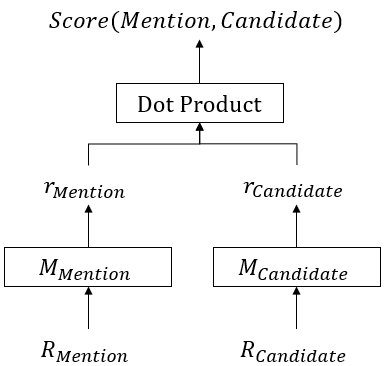
\includegraphics[scale=0.65]{BiencoderB.png}
    \hspace{1.5cm}
    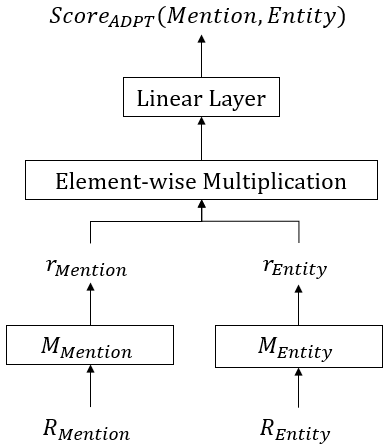
\includegraphics[scale=0.65]{BiencoderADPT.png}
    \caption{BI$_{BL}$ (left) and BI$_{AD}$ (right)}
    \label{fig:biencoderB}
\end{figure}

\subsubsection{BI$_{AD}$}
\label{sec:biencoderadaptexplanation}

Different from BI$_{BL}$, BI$_{AD}$ uses a binary classification setting. For this purpose, a training set is constructed. Every mention and the corresponding correct entity are added with a positive label, and the incorrect entities for a mention are added with a negative label. Hence, the dataset $S$ has the form:

\begin{equation}
    S = \{ (m_k,e_k,l_k) \ | \ l_k \in \{0,1\} \land l_k=1 \iff link(m_k) = e_k \}.
\end{equation}

\noindent where $m_k$ is a mention, $e_k \in \mathcal{E}-\emptyset$ is an entity and $l_k$ is the binary classification label of that sample. To get the class probabilities for each mention and entity pair, an additional linear layer is used. Then, the score of a pair is defined to be the probability of the positive class:

\begin{equation}
    Score_{AD}(\textit{Mention},\textit{ Entity}) = \bold{W}_{AD} \ (r_{Mention} \odot r_{Entity}) [positive]
\end{equation}

\noindent where $\odot$ refers to element-wise multiplication of the vectors, and $\bold{W}_{AD} \in \mathcal{R}^{768x2}$ is a matrix denoting the weights of the additional linear layer\footnote{the size of the final hidden vectors of BERT$_{SC}$ is 768 as it is trained from BERT$_{BASE}$}. The binary cross-entropy loss $L_{AD}$ is used to train this model:

\begin{equation}
    L_{AD}(m_i,e_i,l_i) = - l_i \log (Score_{AD}(m_i,e_i)) - (1-l_i) \log (1-Score_{AD}(m_i,e_i)).
\end{equation}

To get incorrect (negative) entities for each mention, a different strategy is used. For the initial round of training, Neg$_{R}$ entities are sampled from the entity set for each mention randomly. Here, Neg$_{R}$ is a hyperparameter. As Neg$_{R}$ increases, the size of the dataset increases and hence the training becomes longer. Even though in-batch negatives are much faster to use, the advantage of this strategy is the possibility to show the model some entities that do not have any correct mention in the KB. Since the entity distribution of the dataset used is highly skewed (see Figure \ref{fig:entpopul}), it is inevitable that the same entities are used as the random negatives for most of the mentions when in-batch negatives are used.

As in BLINK, hard negatives are defined as the top Neg$_{H}$ entities predicted for a given mention. Different from BLINK, following \cite{googleintern}, an entity is considered to be a hard negative only if it is ranked above the correct entity. Hence, some mentions may have less hard negative samples compared to others. NIL mentions always have Neg$_{H}$ number of hard negative samples. One may argue that the entities that have a score lower than 0.5 should not be considered as a hard negative since they are predicted as the negative class, empirical results suggested that adding such entities helped. Another advantage of this setting is, since hard negatives are not added to the random negatives for loss calculation, it is possible to increase Neg$_{H}$ without the need for additional memory.

The training is done in rounds, similar to BLINK (and BI$_{BL}$) and \cite{googleintern}. In each round, a new set of hard negatives and random negatives are sampled, hence the training set is updated. However, hard negatives are added starting from the second round, as initially some of the model weights are initialized randomly, such as $\bold{W}_{AD}$. In this work, one round may correspond to one or more epochs (see Section \ref{sec:EvalExpSetupTraining})

The number of random negatives in each round, Neg$_R$ is also a hyperparameter. In the first round of training, Neg$_R$ is set to 3 as the training time increases proportionally with Neg$_R$. In the following rounds, Neg$_R$ is selected based on the number of hard negative samples. After extracting all the hard negatives for the training set, the total number of such samples are calculated, which can be denoted as $Neg_{H}^{Sum}$. Then for each mention, $Neg_R = \lfloor Neg_{H}^{Sum}/ \text{(Number of Mentions)} \rceil$ entities are sampled randomly and added to the dataset. This way, it is aimed to have a similar proportion between random and hard negatives in the training set. The aim with this was to somehow mimic the strategy of \cite{googleintern}, which uses a multi-task learning setup with equal weights to incorporate both hard and random negatives. 

One interesting property of the setup of BI$_{AD}$ is that for the mentions with more hard negatives, i.e. mentions that are ranked lower by the model, the training set has more hard negatives compared to random negatives. We hypothesize that the need for hard negatives are higher for these kind of mentions, as it seems that the random negatives were not enough to teach the model to make the correct decision in the first round.

In the setup for BI$_{AD}$, it is intuitive to add NIL mentions to training. The only difference between a NIL mention and a non-NIL mention is the former not having any instance in the training set with a positive label. Also, when BI$_{AD}$ is used as an ED system by itself, it is straightforward to detect NIL mentions. Since this is a binary classification task, if the highest scoring entity of a mention has a score lower than 0.5, it should be a NIL mention, as there are no mention-entity pairs including that mention such that the label is positive. 

The architecture of BI$_{AD}$ is shown in Figure \ref{fig:biencoderB} (right).

\subsubsection{Candidate Reranking}
Instead of using the computationally expensive cross-encoder, a logistic regression model is used as a reranker. After selecting the best biencoder, the number of candidates $K$ is determined by investigating the change of recall with respect to the rank. After $K$ is selected, a training dataset is created by extracting the top $K$ entities for each mention. For the instances where the entity is the correct link for the mention, the class label is set to positive, and for the other instances, it is set to negative.

A feature-based ED model is used for evaluation to compare with the neural approaches. This model uses BM25 \cite{bm25} scores for selecting a candidate set and a Gradient Boosted Machine (GBM) \cite{GBM} with 26 features for reranking. The candidate selectors extracts a maximum of 20 entities and has a coverage of 94\%. This model is referred to as GBM$_{F26}$.

As features to the linear reranker, the ones that had the highest importance in the feature-based model are used: score assigned by the candidate selector, maximum sorted Levenshtein similarity between the mention and the labels of the candidate entity, popularity of the candidate entity, link probability of the mention, and commonness. To calculate Levenshtein similarity, the normalized Levenshtein distance is subtracted from 1. For calculating the maximum sorted Levenshtein similarity for a given mention and entity, first the mention and the labels of the entity are tokenized. Then, the tokens of the mention and each label are sorted in alphabetic order. Levenshtein similarity is calculated between the mention for each entity label. The value of the feature is set to the maximum of these similarities. The sorted Levenshtein similarity is calculated using the Fuzzywuzzy library\footnote{\url{https://github.com/seatgeek/fuzzywuzzy}}.

The popularity of an entity is defined as the number of times it appears as a link divided by the number of all links. Similarly, the link probability \cite{balog} of a mention is defined as the number of times the mention is linked to any entity in the KB divided by the number of times it appears in the dataset used for estimation. Commonness measures the maximum likelihood probability of an entity being the link to the given mention \cite{balog}. For a mention-entity pair, it is calculated as number of times that the mention was linked to the given entity, divided by the number of times that the mention appears as a link \cite{balog}. For popularity, link probability and commonness, the statistics used by the feature-based ED model is utilized. It is made sure that no document that is contained in the evaluation dataset (Dev, Validation and Test splits, see Section \ref{sec:EvalExpSetupData}) is included in the estimation of these statistics.

In the training data, the negative class is prominent as there is only a maximum of one positive entity per mention. To address this, class weights are used during the binary cross-entropy loss calculation. Each class is assigned a weight that is inversely proportional to the number of samples of that class in the training data normalized by the total number of samples. Two hyperparameters of the logistic regression model is tuned by grid search: the regularization strength and the ratio between L$_1$ and L$_2$ penalties. For the former, the search interval is set to [0,1] with a step size of 0.1, and for the latter, it is set to [1,10] with a step size of 1. Feature selection is also performed on all possible feature sets, excluding the ones that do not contain the score of the candidate selector as feature. Then, the best hyperparameter configuration and feature set is selected.

During inference, the probability of the positive class is extracted for each mention-candidate entity pair. The mention is linked to the candidate entity with the highest score, if the score is greater than or equal to 0.5. Otherwise, the mention is linked to NIL. For experimental purposes, another NIL-mention detection threshold is selected within the interval [0.5,1] with using grid search with a step size of 0.001. 

The linear reranker will be denoted by LM which stands for \textit{Linear Model}. For comparison reasons, a GBM model is trained with the same features LM is using. This model will be referred to as GBM$_{F5}$ as it uses 5 features. The hyperparameters used for this model can be found in Appendix \ref{app:lgbm}.


\newpage
\chapter{Evaluation}
\label{sec:Evaluation}
In this work, different experiments were conducted to investigate the optimal Entity Linking (EL) approach for funding information extraction. First, BERT$_{SC}$, a BERT model that is adapted to funding text, is pretrained using the Task-Adaptive Pretraining (TAPT) strategy proposed by \cite{DontStop}. Then, different state-of-the-art Named Entity Recognition (NER) components are compared and a neural Entity Disambiguation (ED) model is developed. Lastly, the end-to-end EL performance of these approaches are investigated.

In Section \ref{sec:EvalExpSetup}, the experimental setup is presented. The dataset used and the evaluation metrics are detailed in Section \ref{sec:EvalExpSetupData} and \ref{sec:EvalExpSetupEval} respectively. The training, hyperparameters and model selection is shown in Section \ref{sec:EvalExpSetupTraining}. Lastly, the result and the analysis are presented in Sections \ref{sec:EvalResults} and \ref{sec:EvalAnalysis}.

\section{Experimental Setup}
\label{sec:EvalExpSetup}

\subsection{Data}
\label{sec:EvalExpSetupData}

The dataset for funding data extraction and the knowledge base (KB) for ED used in this research is provided by Elsevier B.V.. The dataset consists of a set of labelled articles annotated by humans. To create this dataset, each article is annotated by three people. First, two annotators extracted the funding information from the articles independently. Then, a third annotator harmonized the decisions of the previous two annotators, resolving the conflicts if necessary. 

For developing models and evaluating various approaches, the dataset is divided into four subsets: Training, Dev, Validation and Test. The Training split is used to train the models. Dev split is used to monitor the progress of training, while Validation split is used to select the best approach for each task. The intermediate error analyses are done on the Dev split. Test is used to evaluate only the feature-based models and the selected approach for each task. The splits are arranged such that there is no overlap in terms of articles. Table \ref{tab:goldstats} shows the number of annotated articles contained in each split.

\begin{table}[h!]
    \centering
    \begin{tabular}{c c}
    Dataset Split  & Number of Articles  \\
        \hline
    Training &  37,484\\
    Dev & 1,000\\
    Validation & 4,000\\
    Test & 19,920 \\
    \end{tabular}
    \caption{Number of annotated articles in each dataset split}
    \label{tab:goldstats}
\end{table}

For the ED and EL task, the KB provided by Elsevier is used. This KB contains 26,892 entities of funding organizations with information such as the country of origin, type of organization and different names that the organization can be referred to with. There are also sparse amount of relations between organizations to show affiliations and hierarchies. One interesting property of the KB is that most of the entities do not exist in general-purpose knowledge repositories. Hence, it is not trivial to obtain more information from other sources.

Sometimes, organizations may change their names, or may be merged with other organizations. Hence, it is possible that one funding organization is referenced by multiple entities in the KB, which is not desirable. To prevent this, entities are grouped together based on the relations indicating such cases. This operation resulted in 25,859 entity groups. It is assumed that the entities in each group refer to the same organization, and hence can be used interchangeably. Another option could be to only keep the newest versions of the entities. However, this may cause problems with disambiguating older publications, where the authors may have used an older name variant to refer to the same organization.

The data to train and evaluate the approaches for different tasks are derived from this main dataset. However, as each task has a different nature, some preprocessing and filtering is applied when necessary. 
%\newline
%\newline
%\textit{\textbf{Task-Adaptive Pretraining %(TAPT):}}
\subsubsection{Task-Adaptive Pretraining (TAPT)}
For EL in funding domain, the input text is the sentences where the authors acknowledge the funding support they had received for their research. As TAPT can be done with unlabelled data, 13 million such sentences are extracted from Scopus, where they are displayed for each article. Using the identifiers of the articles, the sentences belonging to the articles in Dev, Validation and Test splits are removed.
%\newline
%\newline
%\textit{\textbf{Named Entity Recognition (NER):}}
\subsubsection{Named Entity Recognition (NER)}
As mentioned in Section \ref{sec:NERMEThod}, IOB tagging is used to train and evaluate the NER models. In the dataset used for this work, the annotations are not done in terms of tokens, but in terms of character spans of the input text. That is, each gold mention is provided using their character offsets with respect to the article text. Hence, first the input text is tokenized and the labels are assigned to tokens based on some predefined rules to tackle some edge cases that mostly correspond to annotation errors. These rules are extracted based on empirical results to maximize the correctness of the annotations. The experiments were done on a portion of the training set, and all the edge cases found were present for less than $0.5\%$ of the investigated dataset. In Appendix \ref{app:NERPrepro} the details of the labeling step can be found.

\begin{table}[h!]
    \centering
    \begin{tabular}{ccccc}
    Dataset &  &  &\#ORG& \#GRT  \\
    Split & \#Articles & \#Sentences &Mentions&Mentions \\
    \hline
    Training   &22,720&26,132& 67,671 &45,263 \\
    Dev &1,000&1,284&4,333&2,770\\
    Validation &4,000&5,012&16,355 & 10,112\\
    Test & 13,851 & 15,590 &37,495&25,349\\
    \end{tabular}
    \caption{Dataset splits and statistics for NER. For each split; number of articles with at least one funding sentence, number of sentences and number of mentions are shown.}
    \label{tab:goldstatsner}
\end{table}

The NER component should extract the mentions of organizations only if they funded the corresponded research. For this purpose, the classifier developed by Elsevier is used as a preprocessing step. This classifier identifies whether a sentence contains funding information or not. As the NER component will directly work with this classifier, as a preprocessing step, the dataset splits are reduced to the sentences that are identified as positive by this classifier. The second column of Table \ref{tab:goldstatsner} shows the number of articles with at least one sentence with funding information for each dataset split, and the third column shows the total number of such sentences. Furthermore, the number of organization and grant mentions on each split can be found in the fourth and fifth columns respectively. In Figure \ref{fig:nerdatalen}, the distribution of number of characters for the sentences and mentions contained in the Training and Dev splits are presented.


\begin{figure}
    \centering
    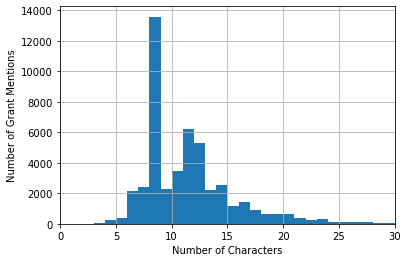
\includegraphics[scale=0.45]{grant_lens.png}
    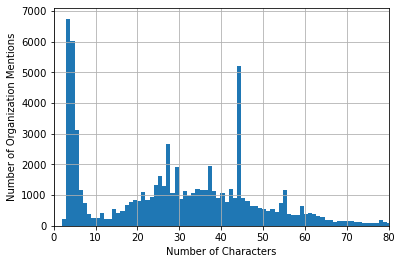
\includegraphics[scale=0.45]{org_lens.png}
    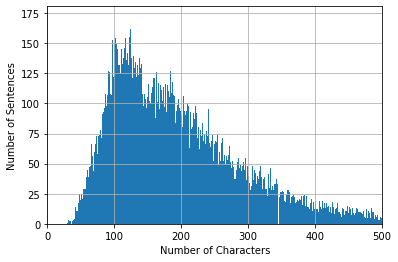
\includegraphics[scale=0.45]{sentence_lens.png}
    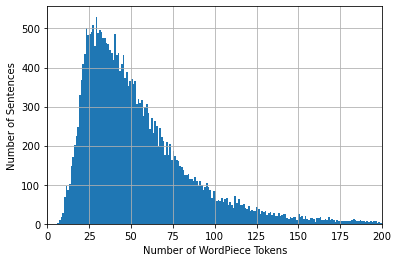
\includegraphics[scale=0.45]{sentence_tokens.png}
    \caption{Distribution of length of grant mentions (top-left), organization mentions (top-right), sentences (bottom-left) in terms of number of characters and distribution of number of tokens per sentence (bottom-right). Plots are cut over the x-axis, and the maximum x values are 75, 223, 9175 and 2760 respectively.}
    \label{fig:nerdatalen}
\end{figure}

%\noindent \textit{\textbf{Entity Disambiguation (ED):}} 
\subsubsection{Entity Disambiguation (ED)}
For this task, the whole dataset is used. Table \ref{tab:goldstatsed} displays the statistics for each dataset split. The second column of this table shows number of articles with at least one organization mention. It also can be seen that not all organization mentions have a corresponding entity in the KB. These mentions will be referred to as NIL mentions. A mention being NIL means that a funding organization is extracted by the annotators, however, as this organization was not yet included in the KB, it was not linked. Because of this, all NIL mentions for this task can be classified as emerging entities (EE). These are very important for this work, as the current KB is being updated regularly consulting to the detected EEs.

\begin{table}[h!]
    \centering
    \begin{tabular}{ccccc}
    Dataset Split & \#Articles & \#ORG Mentions & \#Links & NIL Mentions  \\
    \hline
    Training & 29,118 & 95,761 & 77,972 & 18.58\% \\
    Dev & 991 & 5,618 & 4,749 & 15.47\% \\
    Validation & 3,943 & 19,765 & 16,689 & 15.56\% \\
    Test & 17,333 & 52,378 & 42,514 & 18.83\% \\ 
    \end{tabular}
    \caption{Dataset splits and statistics for ED. For each split, number of articles with at least one organization mention, number of organization mentions, number of mentions that are linked to an entity and the percentage of NIL mentions are shown.}
    \label{tab:goldstatsed}
\end{table}

Another interesting property of this dataset is that only the entities belonging to a small part of the KB appear as a link, as can be seen from Table \ref{tab:goldstatsed2}. For example, only 26.9\% of the entities in the KB appear as a link in the Training split. In addition, the  Dev, Validation and Test splits contain links to entities that do not appear in the Training split. However, when  Table \ref{tab:goldstatsed3} is investigated, it is possible to see that such instances are long-tail entities. For example, even though 28.1\% of the unique entities in the Test split do not appear in the Training split; when the overall number of links are checked, only 5.14\% of the links are to these entities. Nevertheless, it is important that the ED system can link mentions of unseen entities correctly as well.


Figure \ref{fig:entpopul} shows the number of occurrences of the top 25 most frequent entities on Training and Dev splits. It can be seen that the distribution is highly skewed, even with the most common entities. 

\begin{table}
    \centering
    \begin{tabular}{cccc}
    Dataset Split & \# Unique Entities & Overlap with Training & KB Coverage\\
    \hline
    Training & 7,234 & - & 26.9\%\\
    Dev & 1,222 & 88.63\% & 4.54\%\\
    Validation & 2,658 & 81.6\% & 9.88\%\\
    Test & 5,590 & 71.91\%& 20.79\%\\
    \end{tabular}
    \caption{Dataset splits and number of unique entities in each split. Third column indicates the percentage of unique entities that are also present in the Training split for Dev, Validation and Test splits. The last column shows the percentage of KB covered by each split.}
    \label{tab:goldstatsed2}
\end{table}

\begin{table}
    \centering
    \begin{tabular}{ccc}
    Dataset Split & \# Links & Links not in Training\\
    \hline
    Dev & 4,749 & 3.39\% \\
    Validation & 16,689 & 3.52\% \\
    Test & 42,514 & 5.14\% \\
    \end{tabular}
    \caption{Dataset splits and number of links. The third column shows the percentage of links for which the target entity do not exist as a link in the Training split.}
    \label{tab:goldstatsed3}
\end{table}

\begin{figure}
    \centering
    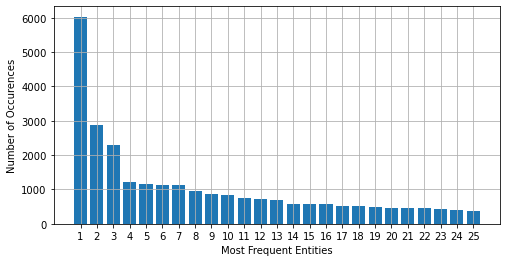
\includegraphics[scale=0.6]{ent_occ.png}
    \caption{Number of occurrences of top 25 most frequent entities. Statistics obtained using Training and Dev splits.}
    \label{fig:entpopul}
\end{figure}


%\noindent \textit{\textbf{Entity Linking (EL):}} 
\subsubsection{Entity Linking (EL)}
In this work no end-to-end EL system is trained as the task of EL is tackled in two-steps, NER and ED. Hence, the data described is used to evaluate the end-to-end performance of an NER and an ED system put together. 

As the NER is also evaluated here implicitly, the Sentence classifier is used again to limit the dataset to the sentences detected by this classifier, as done for the NER task dataset. Also, all the NIL mentions are classified as emerging entities, due to the same reason reported for the ED task dataset. In fact, the dataset for EL is a subset of that of ED, limited by the sentence classifier. Tables \ref{tab:goldstatsel}, \ref{tab:goldstatsel2} and \ref{tab:goldstatsel3} show statistics of the dataset splits such as number of mentions, links and percentage of NIL mentions.

\begin{table}[H]
    \centering
    \begin{tabular}{ccccc}
     Dataset Split & \#Articles & \#ORG Mentions & \#Links & NIL Mentions  \\
     \hline
    %Dev & 1,000  & 4,622 & 3,954  & 14.45\% \\
    Validation & 4,000  & 16,276 & 13,958 & 14.24\% \\
    Test           & 13,851 & 37,340 & 31,153 & 16.57\% \\
    \end{tabular}
    \caption{Dataset splits and statistics for EL. For each split, number of articles with at least one organization mention, number of organization mentions, number of mentions that are linked to an entity and the percentage of NIL mentions are shown.}
    \label{tab:goldstatsel}
\end{table}


\begin{table}[H]
    \centering
    \begin{tabular}{cccc}
    Dataset Split & \# Unique Entities & Overlap with Training & KB Coverage\\
    \hline
    %Dev & 1,034 & 89.46\% & 3.85\%\\
    Validation & 2,302 & 83.36\% & 8.57\%\\
    Test & 4,350 & 76\%& 16.18\%\\
    \end{tabular}
    \caption{Dataset splits and number of unique entities in each split. Third column indicates the percentage of unique entities that are also present in the Training split. The entities in the Training split is determined using the dataset for the ED task. The last column shows the percentage of KB covered by each split.}
    \label{tab:goldstatsel2}
\end{table}

\begin{table}[H]
    \centering
    \begin{tabular}{ccc}
    Dataset Split & \# Links & Links not in Training\\
    \hline
    %Dev & 3,954   & 3.14\% \\
    Validation &  13,958 & 3.19\% \\
    Test &            31,153 & 4.28\% \\
    \end{tabular}
    \caption{Dataset splits and number of links. The third column shows the percentage of links for which the target entity do not exist as a link in the Training split. The entities in the Training split is determined using the dataset for the ED task.}
    \label{tab:goldstatsel3}
\end{table}

\subsection{Evaluation Metrics}
\label{sec:EvalExpSetupEval}
Each different problem tackled in this work is evaluated with a suitable metric selected from the literature.
%\newline
%\newline
%\textit{\textbf{Task-Adaptive Pretraining (TAPT):}} 
\subsubsection{Task-Adaptive Pretraining (TAPT)}
To evaluate BERT$_{SC}$ and monitor its progress, Perplexity is used. This metric corresponds to the inverse probability of the dataset based on the model \cite{perplexity}, and it it is the most popular metric to evaluate language models \cite{perplexity}. 
%\newline
%\newline
%\textit{\textbf{Named Entity Recognition (NER):}}
\subsubsection{Named Entity Recognition (NER)}
To evaluate the NER task, precision recall and F1 scores are used for each entity type, Organization and Grant. These metrics are defined in terms of True Positives (TP), False Positives (FP) and False Negatives (FN). Precision is defined as the fraction of TPs among all mentions extracted by the system, and recall is defined as the fraction TPs among all ground truth mentions. F1 score is the harmonic mean of precision and recall metrics. The formulas of these metrics are shown in Equations \ref{eq:pr},\ref{eq:re} and \ref{eq:f1}. A mention is considered to be a TP if and only if both the extracted span and type information is correct. A FP corresponds to a mention that is extracted by the system wrongly, and a FN corresponds to a mention that is not extracted by the system while being present in the ground truth. This scheme is chosen as it is inline with evaluation of the CoNLL-2003 NER task \cite{conll}.

\begin{equation}
\label{eq:pr}
    \text{Precision} = \frac{\#TP}{\#TP+\#FP} 
\end{equation}
\begin{equation}
\label{eq:re}
    \text{Recall} = \frac{\#TP}{\#TP+\#FN} 
\end{equation}
\begin{equation}
\label{eq:f1}
    \text{F1 Score} = \frac{2\cdot\text{Precision}\cdot\text{Recall}}{\text{Precision}+\text{Recall}} 
\end{equation}

%\newline
%\newline
%\textit{\textbf{Entity Linking (EL):}} 
\subsubsection{Entity Linking (EL)}
To evaluate the EL task, a strategy inspired by GERBIL \cite{gerbil} is used. GERBIL is a framework for evaluating various entity-related tasks, such as NER, ED and EL. The framework supports many popular databases, hence, systems evaluating on such datasets can use it when they provide an API support. However, since this work is using a domain-specific and private dataset, it is not possible to make use of it directly. Hence, the metrics are reimplemented consulting the paper \cite{gerbil} and the GitHub repository\footnote{\url{https://github.com/dice-group/gerbil}}. 

GERBIL offers various settings to evaluate systems. In this work, ``Normal'', ``EE'' (Emerging Entities) and ``InKB'' (In Knowledge Base) settings are used for evaluation and the results for each are reported separately. 

To calculate the scores in ``Normal'' setting, for each document, the TP, FP and FN instances are counted. First, for each gold annotation, a matching annotation is looked for in predictions. Two annotations are considered to be matching based on strict criteria. If a match is found, this counts as a TP. Gold annotations for which no match is found are counted as FN. Similarly, the predictions that were not marked as a match for any gold annotation are counted as FP. If a prediction is marked as a match for a gold annotation, it could not be matched again. And, a gold annotation could not be matched with more than one prediction. After obtaining the TP, FP and FN counts; precision, recall and F1 score for that document are calculated. The precision, recall and F1 score for all the documents are averaged to produce macro averaged results. To obtain micro averaged results; the TP, FP and FN counts of all documents are summed together before calculating precision, recall and F1 score. 

GERBIL distinguishes NIL mentions to two, emerging entities and ones where the system cannot produce a link. In this work, for the ED task, it is known that all NIL mentions are emerging entities, and the systems developed are not able to make such distinction between NIL mentions. Hence, for the EL task, the mentions extracted by the NER components are also assumed to be emerging entities, even though this may not always be the case. Based on this assumption, to get the scores for the ``EE'' setting, the TP counts are discarded when the annotations both contained an entity that is in the KB. The gold annotations that were not matched with any prediction did not count as FN if the entity was in the KB. Similarly, the predictions that were not matched did not count as FP if the entity was in the KB. For the ``InKB'' setting, the TP counts are discarded when the entities were both NIL. The gold annotations that were not matched with any prediction did not count as FN if the entity was NIL. And, the predictions that were not matched did not count as FP if the entity was NIL.
%\newline
%\newline
%\textit{\textbf{Entity Disambiguation (ED):}}
\subsubsection{Entity Disambiguation (ED)}
To evaluate the ED systems, the metrics introduced in \cite{NILMentions} is used. This paper has a similar ``InKB'' and ``EE'' setting with GERBIL. They do not have a ``Normal'' setting, however, they report micro and macro averaged accuracy over the whole samples. In the ``InKB'' and ``EE'' setting, the metrics used are precision, recall and F1 score. In this work, the reason why accuracy is reported in ``Normal'' setting is that, since all NIL mentions are assumed to be emerging entities, precision and recall becomes the same according to GERBIL. Different from \cite{NILMentions}, in the ``EE'' and ``InKB'' settings, micro averaged results are calculated instead of macro. 


\subsection{Training, Hyperparameters and Implementation}
\label{sec:EvalExpSetupTraining}
\todo{I thought of putting this section to Approach chapter but then the evaluation metrics are not defined yet}
To conduct the experiments, the models introduced in Chapter \ref{chapter:Approach} are trained and implemented. For training, the Training split prepared for that specific task is used for each model. The details for all the models are explained below.
%\newline
%\newline
%\textit{\textbf{BERT}}$_{SC}$\textit{\textbf{:}}
\subsubsection{BERT$_{SC}$}
The weights of BERT$_{SC}$ are first initialized with the case-preserving version of BERT$_{BASE}$. Following TAPT, the model is trained end-to-end with the sentences extracted from Scopus, using Masked Language Modeling (MLM). The choice of a case-preserving model is due to the fact that case information can provide important information to the NER task, for example, it is common in English to capitalize organization names. The implementation is based on the GitHub repository of the paper where TAPT was introduced\footnote{\url{https://github.com/allenai/dont-stop-pretraining}} \cite{DontStop}. Throughout training, the progress is monitored on Dev split. The hyperparameters recommended by \cite{DontStop} is used as much as possible. Number of epochs are reduced from the recommended number (100) to 2 as the training set is rather large. It is thought that 1 epoch would be sufficient, and a second epoch would be beneficial to see whether Dev scores would improve with more epochs or not. The batch size is set to 4 due to memory requirements, but using gradient accumulation, an effective batch size of 2048 is maintained as recommended. 

However, the initial setup to train BERT$_{SC}$ could not be performed. According to the initial setup, TAPT was going to be performed for around 13,500 steps in 2 epochs. However, after 2 days of training it was observed that only 1000 steps were finished, and hence, only around 2 million training examples were utilized. Due to the time constraints, it was determined to stop the training at that point. 

After 1000 steps, a perplexity of 2.86 is achieved on the Dev set. Figure \ref{fig:perp} shows the change of perplexity on Dev, recorded every 20 training steps. Based on this plot, we believe that it is possible to obtain a model with higher performance when the training with the full dataset is completed. However, this is left to future work.

The training of BERT$_{SC}$ is done on an NVIDIA Tesla K80 GPU with 12 GB of memory. More details on the hyperparameter configuration can be found in Appendix \ref{sec:app:bertsc}.

\begin{figure}
    \centering
    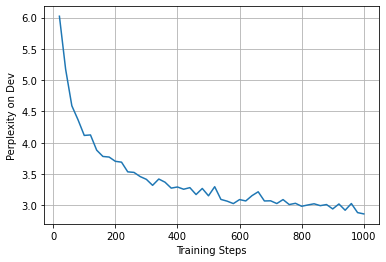
\includegraphics[scale=0.7]{perpplot.png}
    \caption{Perplexity on Dev during training}
    \label{fig:perp}
\end{figure}

%\noindent \textit{\textbf{Flair}}$^{NER}$\textit{\textbf{:}} 
\subsubsection{Flair$^{NER}$}
The implementation of Flair$^{NER}$ is done using the Flair library \cite{flairlib}. In this library, both $LSTM^{forward}_{Flair}$ and $LSTM^{backward}_{Flair}$ trained on the 1 billion word corpus \cite{onebillion} are available. Using these and pretrained GloVe embeddings, the BiLSTM-CRF model is trained on the Training split and the progress is monitored on Dev split using the training interface of Flair.  Mainly, the hyperparameters and training strategy reported in \cite{flairpaper} is followed, while changing minor things to address the computational limitations. 

A batch size of 8 is used, and the model started training with a learning rate of 0.1. When for 2 epochs, no improvement on the Dev split was observed, the learning rate was halved. The training is stopped when no improvement was made in a certain learning rate, amounting to 37 epochs in total. The performance on Dev was measured as micro averaged F1 score of the output tags. The models were saved at the end of each epoch, and the model that performed best on Dev is selected. It was observed that the model at the end of 33 epochs was the best one. The losses, scores and learning rates per epoch are presented in Appendix \ref{sec:app:flairner}. One epoch of training Flair$^{NER}$ took approximately 50 minutes on an NVIDIA Quadro T1000 GPU with 4GB memory. 
%\newline
%\newline
%\textit{\textbf{BERT}}$^{NER}$\textit{\textbf{:}} 
\subsubsection{BERT$^{NER}$}
All parameters of BERT$^{NER}$ are fine-tuned end-to-end with different hyperparameter settings. The progress of training is monitored on Dev across epochs, with respect to the same evaluation metric of the NER task.

Devlin et al. (2019) \cite{BERT} suggested different hyperparameter settings for fine-tuning BERT: a batch size of 16 or 32, learning rate of $5\times10^{-5}$, $3\times10^{-5}$ or $2\times10^{-5}$; and training for 2, 3 or 4 epochs. Due to memory requirements, the batch size is set to 8. Then, the model is trained for 10 epochs with a learning rate of $2\times10^{-5}$, while saving the model at the end of each epoch. On top of that, 3 more models are trained using a linear learning rate scheduler for 2, 3 and 4 epochs respectively. The number of warm-up steps is set to 50. For implementation, the library Transformers \cite{huggingface} by Hugging Face\footnote{\url{https://huggingface.co/}} is used.

After the experimentation with different hyperparameter settings, it was decided that training for 3 epochs with a linear learning rate scheduler produced the best results. Appendix \ref{sec:app:bertner} shows detailed results on this experimentation.

BERT$^{NER}$ can process a maximum of 512 tokens per input, similar to BERT$_{BASE}$. Hence, the sentences having more tokens are split into smaller chunks, such that there is no overlap between chunks and no word is scattered across chunks. Later on, the predictions are merged as a postprocessing step. The training is done using an NVIDIA Tesla K80 GPU with 12 GB of memory. On this device, one epoch took approximately 1 hour. 
%\newline
%\newline
%\textit{\textbf{BERT}}$^{NER}_{SC}$\textit{\textbf{:}} 
\subsubsection{BERT$^{NER}_{SC}$}
BERT$^{NER}_{SC}$ is trained with the exact same hyperparameter settings that produced the best results for BERT$^{NER}$, i.e. for 3 epochs with a linear learning rate scheduler.

One aim of this study is showing the effect of domain adaptation, which is achieved by comparing BERT$^{NER}$ and BERT$^{NER}_{SC}$. To be able to show that the improvement gained by pretraining is not random, a second BERT$^{NER}_{SC}$ is trained with the second-best hyperparameter setting, for 2 epochs with a linear learning rate scheduler. However, the aim of this second BERT$^{NER}_{SC}$ is just for observing the effect of domain adaptation, not for measuring the success of any other task. Hence, when BERT$^{NER}_{SC}$ is referred to in any other setting, it is the one trained for 3 epochs.

BERT$^{NER}_{SC}$ can also process a maximum of 512 tokens, and is also trained on the same GPU with BERT$^{NER}$. One epoch of training took approximately 1 hour.
%\newline
%\newline
%\textit{\textbf{Biencoder}}$_{B}$\textit{\textbf{:}} 
\subsubsection{BI$_{BL}$}
The implementation of BI$_{BL}$ is inspired by BLINK's GitHub repository\footnote{\url{https://github.com/facebookresearch/BLINK/tree/master/blink}}. Mainly, the code for data preprocessing is obtained from this repository. The models and training are implemented using PyTorch \cite{pytorch} and Transformers library by Hugging Face.

As there was no computational power to be able to do an extensive hyperparameter search, the values reported by \cite{scalablezeroshot} is followed as much as possible. In BLINK, the maximum number of tokens for the mention representation ($R_{Mention}$) are either 32 or 128, depending on the dataset. This number is set to 64 in this work. Originally it was planned to set it to 32 to address the memory limitations, however, it was observed that there were mentions longer than 32 tokens themselves.

For candidate representation ($R_{Entity}$), BLINK uses 128 tokens. However, in this setting, there are candidates that have longer representations. To be more specific, there are 96 entities with representation longer than 128 tokens, 36 entities longer than 256 tokens, and 23 entities longer than 256. Hence, for the 96 entities that had longer representations, a label is removed iteratively until the representation was equal to or shorter than 128 tokens. The label that had the highest sorted Levenshtein distance with any other label is removed in each iteration, as it was thought that this label would be the least informative.

BLINK uses a batch size of 128, and adds 10 hard negatives (Neg$_H$=10) among the in-batch negatives. Hence, for a mention, they make use of a maximum of 127 random negatives, and a maximum of 137 negatives in total ($max(|IE|)=127+10=137$). As the training is done on a GPU with 12 GB memory, this batch size could not be maintained in terms of random negatives. Hence, the hyperparameters are scaled down proportionally. It was observed that a maximum batch size of 16 was possible. Proportionally, Neg$_H$ is set to 1, making $max(|IE|)=15+1=16$.

Even though a batch size of 128 cannot be maintained in terms of in-batch random negatives, it is possible to maintain this number in terms of gradient updating using gradient accumulation. Initially, the batch size was set to be inline with BLINK. Similarly, the learning rate was set to $10^{-5}$. However, no learning was observed with this setting. We hypothesize that it is because of the size of the dataset. At the end, the batch size is set to 64 using gradient accumulation and the learning rate is set to $2 \times 10^{-5}$, which is also the minimum learning rate recommended by \cite{BERT}.

The models in BLINK are trained for either 4 or 5 epochs. It is not clear whether the hard negative sampling is done for each epoch or not. However, as they report that they are following the strategy of \cite{googleintern}, it will be assumed that one epoch corresponds to one round for this case. Based on this, initially, it was thought to have 4 rounds of training, each consisting of 1 epoch. No hard negatives are added in the first round, as some weights of the model are initialized randomly anyway. To observe the course of training and the change in performance after each round, Dev is used.

Table \ref{tab:biencoderbres} shows the performance of BI$_{BL}$ on Training and Dev sets after the first two rounds. It can be seen that after the second round, the performance drops further for the ``InKB'' setting but improves for the ``EE'' setting, resulting in an overall performance decline as shown with accuracy. We hypothesize that the second round of training resulted in better separation of the scores of NIL and not-NIL mentions, however, did not improve the model in terms of finding the correct entity. 


\begin{table}
    \centering
    \begin{tabular}{cccc}
    &&Micro Averaged & Macro Averaged\\
    Round    & Dataset & Accuracy &Accuracy \\
    \hline
    1  & Training & 61.88&62.9\\
    2  & Training & 59.2&	59.21\\
    1  & Dev & 60.16	&64.04\\
    2  & Dev & 55.06	&59.13\\
    \end{tabular}
    
    \vspace{0.5cm}\begin{tabular}{ccccc}
    &&&EE Setting & \\
    Round    & Dataset & Precision & Recall & F1 Score \\
    \hline
    1  & Training &60.32&	60.64&	60.48 \\
    2  & Training &64.42&	85.03&	73.3 \\
    1  & Dev &50.4&	57.31&	53.63 \\
    2  & Dev &54.1&	72.96&	62.13\\
    \end{tabular}
    
    \vspace{0.5cm}\begin{tabular}{ccccc}
    &&&InKB Setting & \\
    Round    & Dataset & Precision & Recall & F1 Score \\
    \hline
    1  & Training &62.24&62.16	&62.2\\
    2  & Training &57.51&53.31	&55.33\\
    1  & Dev &62.25&60.69	&61.46 \\
    2  & Dev &55.31&51.78	&53.49\\
    \end{tabular}
    
    \caption{Scores of BI$_{BL}$ for the first two rounds. A threshold of 0.324 is used for the first and 0.321 for the second round.}
    \label{tab:biencoderbres}
\end{table}

To see the separation between NIL mentions and non-NIL mentions, it is possible to model the distribution of scores. For this purpose, two normal distributions are fit on the normalized scores (see Section \ref{sec:biencoderbexplanation} for details of the normalization) of the highest ranked entity for each mention, one for NIL mentions and one for others. The parameters of the distribution are calculated using Maximum Likelihood and Dev dataset, and are shown in Table \ref{tab:nilnotnilBparams}. Figure \ref{fig:biencoderbnil} shows the histogram of scores for each distribution. When the Bhattacharyya distance  \cite{bhatt} is checked, it is possible to see that the distribution of NIL mention scores are more different than the other mentions in Round 2, compared to Round 1. The choice of this metric is due to the fact that it is reported as a convenient metric to measure the class separability of normal distributions \cite{bhatt}.

\begin{table}
    \centering
    \begin{tabular}{c|cc|cc|c}
    & \multicolumn{2}{c|}{NIL Mentions} & \multicolumn{2}{c|}{Other Mentions} & Bhattacharyya\\
     Round  &  Mean & Std. Dev. &  Mean &  Std. Dev.& Distance\\
     \hline
    1     &  0.311& 0.109&0.465&0.11&0.247\\ 
    2     & 0.263&0.099 & 0.534 & 0.17&0.541\\
    \end{tabular}
    \caption{Parameters of the distributions for scores and the Bhattacharyya distance between the two distributions for each round.}
    \label{tab:nilnotnilBparams}
\end{table}

\begin{figure}
    \centering
    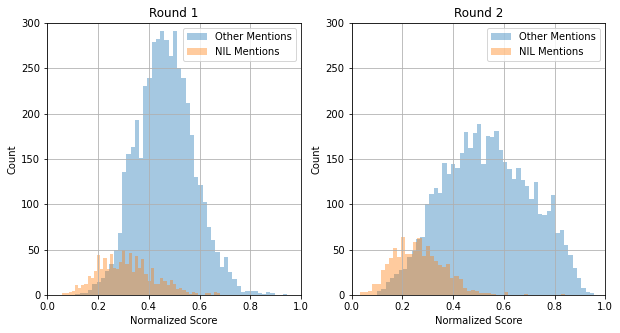
\includegraphics[scale=0.5]{biencoderbnil.png}
    \caption{Distribution of scores for BI$_{BL}$, first two rounds, on Dev.}
    \label{fig:biencoderbnil}
\end{figure}

Based on the results, the training of BI$_{BL}$ is stopped after two rounds, and was not used any further. The training of the first round took 1.3 and the second round took 1.7 hours in the NVIDIA Tesla K80 GPU with 12 GB of memory.
%\newline
%\newline
%\textit{\textbf{Biencoder}}$_{ADPT}$\textit{\textbf{:}} 
\subsubsection{BI$_{AD}$}
To train BI$_{AD}$, the same batch size and learning rate with that of BI$_{BL}$ is used. The progress of the training is also monitored using the Dev split. 

The model is trained for 4 rounds, each consisting of one epoch. The initial round of training is done just with random negatives, and Neg$_R$ is set to 3. This hyperparameter is not tuned as there is not much performance improvement expected from the initial round. It could be that a higher Neg$_R$ leads to a better result, however, the training time would also increase accordingly. In the following rounds, Neg$_H$ is set to 10, as BLINK also uses 10 hard negatives. Based on the formula introduced in Section \ref{sec:biencoderadaptexplanation}, Neg$_R$ is set to 3, 2 and 2 for the second, third and fourth rounds respectively. Also, in the initial round, class weights are used for loss calculation to prevent the model to predict everything as the negative class. According to the random negative sampling strategy, a weight of 0.25 is given to the negative class and 0.75 is given to the positive class. However, class weights are not used in the following rounds, even though the class imbalance continues. During training, it was seen that not using class weights was slightly better for the performance. This could be because in these rounds the negative samples are selected with hard negative mining, and hence are very informative.

Table \ref{tab:hardnegsbiencoder1} (upper) shows the number of hard negatives for Training and Dev splits after each round. As can be seen, the mentions with no hard negatives increase significantly after the second round, and this increase becomes much smaller in the following rounds. In this setting, the training took around 5, 8.5, 6.5 and 6.5 hours for the first, second, third and fourth rounds respectively; using the NVIDIA Tesla K80 GPU with 12 GB of memory.

\begin{table}
    \centering
    \hspace*{-1.2cm}\begin{tabular}{ccccccccccccc}
    Dataset  & Round & None & 1 & 2 & 3 & 4 & 5 & 6 & 7 & 8 & 9 & 10+ \\
    \hline
    Training & 1 & 51,482&12,711&4,470&1,873&1,244&1,034&691	&517&	450&356&3,144\\
    Training & 2 & 70,566&3,024	&916&	516	&327	&194&	147&	135	&133&	104&1,910\\
    Training & 3 & 71,547&3,329	&899&	402	&272	&187&	153&	102&	88&	85&908\\
    Training & 4 & 73,273&2,273	&821&	313	&200	&117&	85	&57	&62&	53&718\\
    \hline
    Dev & 1 & 3,063&771&283&	122&63	&63	&49&	36	&17&	30&252\\
    Dev & 2 &4,204&173&58	&36&24&	6	&12&	12	&12&	5 &207\\
    Dev & 3 & 4,222&212&74&	33&19	&10	&14&	12&	9&	5&139\\
    Dev & 4 & 4,291&148&64&	24&13	&12	&13&	5&	9&	10 &160\\
    \end{tabular}
    
    \vspace*{0.5cm}\hspace*{-1cm}\begin{tabular}{ccccccccccccc}
    Dataset  & Round & None & 1 & 2 & 3 & 4 & 5 & 6 & 7 & 8 & 9 & 10+ \\
    \hline
    Training & 1 & 59,711&9,356&2,787&1,559&907&794&436&326&263&205&1,628\\
    Training & 2 & 73,259&2,562&579&374&180&115&100&66&48&42&647\\
    Training & 3 & 74,484&2,141&484&252&152&79&68&45&33&17&217\\
    Training & 4 & 75,403&1,875&295&107&60&38&31&17&9&14&123\\
    \hline
    Dev & 1 & 3,574&556&161&99&49&57&20&25&15&14&179\\
    Dev & 2 &4,288&183&43&31&12&12&11&10&5&3&151\\
    Dev & 3 &4,355&159&51&32&14&20&12&8&4&6&88\\
    Dev & 4 &4,354&178&37&13&7&11&11&8&6&3&121 \\
    \end{tabular}
    
    \caption{Number of not-NIL mentions with \{None, 1,2,...,9 ,10 or more\} hard negatives in each round for BI$_{AD}$. Upper table is with the \textbf{first} set of hyperparameters, and lower table is with the \textbf{second} set of hyperparameters.}
    \label{tab:hardnegsbiencoder1}
\end{table}


As a second set of hyperparameters, it was tried to train each round for 2 epochs instead of one. Also, the maximum tokens for $R_{Entity}$ is set to 256. It was thought that a longer representation would be better in the event that new entities would have many labels. The number was not increased to 512, in case the Cross-Encoder of BLINK \cite{scalablezeroshot} would be implemented later on. A separate experiment to see the effect of this increase to the performance was not conducted as the impacted entities cover 2.42 \% of Training, 2.3 \% of Dev, 2.41 \% of Validation and 2.66 \% of Test split for the ED task. There were 1037 samples in Validation split for which BI$_{AD}$ made a mistake when trained with the first hyperparameter configuration, but got the correct answer when trained with the second hyperparameter configuration. Among these samples, in only 10 of them, the correct entity was affected by this change. Lastly, as the entity embeddings are precomputed before inference, this increase does not have any impact on the efficiency.

Apart from number of epochs per round and the maximum tokens for $R_{Entity}$, the other hyperparameters were not changed. During training, following the formula, Neg$_R$ is set to 2 for second, third and fourth rounds. In this setting, the training took around 11, 15, 13.5 and 14 hours for the first, second, third and fourth rounds respectively; using the NVIDIA Tesla K80 GPU with 12 GB of memory.

\begin{table}
    \centering
    \begin{tabular}{cccc}
    &&Micro Averaged & Macro Averaged\\
    Setting & Threshold     & Accuracy &Accuracy \\
    \hline
    1  & 0.5&83.85&87.3\\
    2  & 0.5&86.95&89.9\\
    1  & 0.732&86.61&89.17\\
    2  & 0.728&88.44&90.75\\
    \end{tabular}
    
    \vspace{0.5cm}\begin{tabular}{ccccc}
    &&&EE Setting & \\
    Setting    & Threshold & Precision & Recall & F1 Score \\
    \hline
    1  & 0.5&81.06	&47.85&	60.18\\
    2  & 0.5&84.22&	58.97&	69.37\\
    1  & 0.732&70.38&	76.24&	73.19\\
    2  & 0.728&75.75&	76.27&	76.01\\
    \end{tabular}
    
    \vspace{0.5cm}\begin{tabular}{ccccc}
    &&&InKB Setting & \\
    Setting    & Threshold& Precision & Recall & F1 Score \\
    \hline
    1  & 0.5&84.13&	90.48&	87.19\\
    2  & 0.5&87.29&	92.11&	89.64\\
    1  & 0.732&89.9&	88.53&	89.21\\
    2  &0.728&90.8&	90.68&	90.74\\
    \end{tabular}
    \caption{Comparing the two hyperparameter settings on Validation split.}
    \label{tab:biencoderadaptres}
\end{table}

Table \ref{tab:hardnegsbiencoder1} (lower) shows the number of hard negatives for the second configuration and Table \ref{tab:biencoderadaptres} shows the results on Validation for both hyperparameter settings. Even though a score of 0.5 is a natural threshold for NIL mention detection as the problem is cast as binary classification, a threshold that maximizes the micro averaged accuracy is selected on the Training split using grid search in the interval [0.5,1] with a step size of 0.001. The thresholds 0.732 and 0.728 are selected for first and second hyperparameter settings respectively. Table \ref{tab:biencoderadaptres} compares the results for both the natural and selected thresholds.

It is possible to see that there are more mentions with no hard negatives in general for the second set of hyperparameters. Moreover, all the scores are higher on Validation when the second hyperparameters are used. That is why, it was decided to use the model that is trained for 2 epochs per round and that has a maximum $R_{Entity}$ of 256.

An interesting observation is, a threshold selection is beneficial for NIL mention detection, which is shown by the ``EE'' evaluation setting. This could indicate that the models do not have a full capability of detecting NIL mentions themselves. 

Appendix \ref{sec:app:biencoderadapt} presents more results on Training and Dev splits for each round of training.
%\newline
%\newline
%\textbf{\textit{Reranker}}$_K$:
\subsubsection{LM}
Before training the model, the number of candidates are selected using Dev based on the best BI$_{AD}$. First, top 20 predicted entities are extracted for each non-NIL mention in the dataset. Then, the coverage of each rank is calculated as the number of mentions for which the correct entity is extracted within that rank divided by the number of non-NIL mentions. Table \ref{tab:coverageestimation} shows the coverage of each rank and how much the coverage increase between ranks. The figure next to the table plots the coverage over ranks. The red dot indicates the selected $K$ value, $K=12$. This value is selected as the coverage does not increase for more than 0.1\% in the following ranks.

\begin{table}

	\begin{minipage}{0.5\linewidth}
	\centering
	\begin{tabular}{c|cc}
    K  & Coverage & Increase \\
    \hline
    1   & 91.68\% & - \\
    2   & 95.43\% & +3.75 \%\\
    3   & 96.21\% & +0.78 \%\\
    4   & 96.48\% & +0.27 \%\\
    5   & 96.63\% & +0.15 \%\\
    6   & 96.86\% & +0.23 \%\\
    7   & 97.09\% & +0.23 \%\\
    8   & 97.26\% & +0.17 \%\\
    9   & 97.39\% & +0.13 \%\\
    10  & 97.45\% & +0.06 \%\\
    11  & 97.52\% & +0.06 \%\\
    12  & 97.66\% & +0.15 \%\\
    13  & 97.73\% & +0.06 \%\\
    14  & 97.81\% & +0.08 \%\\
    15  & 97.83\% & +0.02 \%\\
    16  & 97.85\% & +0.02 \%\\
    17  & 97.85\% & +0.0  \%\\
    18  & 97.87\% & +0.02 \%\\
    19  & 97.89\% & +0.02 \%\\
    20  & 97.98\% & +0.08 \%\\
    \end{tabular}
	\end{minipage}\hfill
	\begin{minipage}{0.5\linewidth}
		\centering
		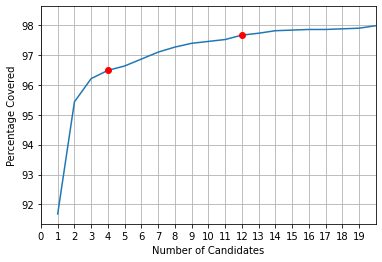
\includegraphics[scale=0.5]{candplot.png}
		\hspace*{-1cm}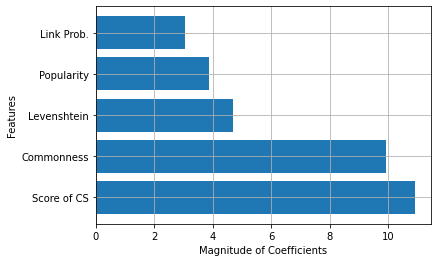
\includegraphics[scale=0.5]{rerankercoef.png}
	\end{minipage}
	\caption{Left: Coverage estimation for each rank on Dev split. Top Right: Coverage plot. Bottom Right: The magnitude of coefficients for LM. Score of CS refers to the score obtained from BI$_{AD}$.}
	\label{tab:coverageestimation}
\end{table}

The best hyperparameter configuration is chosen based on micro averaged accuracy when the NIL mention detection threshold is 0.5. The best feature set included all features, the L$_1$ penalty ratio is set to 0.5 and the regularization strength is set to 10. Figure in Table \ref{tab:coverageestimation} shows the magnitude of coefficients for LM. A NIL mention detection threshold is selected on the interval [0.5,1] using grid search with a step size of 0.001 that maximizes the micro averaged accuracy on Training split. The best threshold remained to be 0.5. It is hypothesized that a lower threshold could perform even better, but is not tried as a score lower than 0.5 would indicate an entity to be classified as negative by the classifier.

\section{Results}
\label{sec:EvalResults}
The results for NER, ED and EL are presented in this section. Different approaches are compared on the Validation splits, and the best performing approach is compared with feature-based models of that task on the Test split.
%\newline
%\newline
%\textit{\textbf{Named Entity Recognition (NER) and Task-Adaptive Pretraining (TAPT):}}
\subsubsection{Named Entity Recognition (NER) and Task-Adaptive Pretraining (TAPT)}


\begin{table}
    \centering
    \begin{tabular}{c| c c c| c c c}
    &\multicolumn{3}{c|}{Organization}&\multicolumn{3}{c}{Grant} \\
    System&Precision&Recall&F1&Precision&Recall&F1\\
    \hline
    Stanford NER & 73.7&	75.1&74.39&94.11&94.77&94.44
 \\[0.7ex]
    BERT$^{NER}$ & 79.18&\textbf{86.03}&\textbf{82.46}&94.71&\textbf{97.39}&96.03
\\[0.7ex]
    BERT$^{NER}_{SC}$ & \textbf{80.28}&\textbf{86.54}&\textbf{83.29}&\textbf{94.9}	&\textbf{97.63}&\textbf{96.24}
  \\[0.7ex]
    Flair$^{NER}$& \textbf{85.83}&78.02&81.74&\textbf{97.56}&95.24&\textbf{96.39}
 \\[0.7ex]
    \end{tabular}
    \caption{NER Results on Validation split}
    \label{tab:all_ner_results}
\end{table}

To compare the developed NER models Stanford NER \cite{stanfordNER} is used as a feature-based model. Table \ref{tab:all_ner_results} compares the precision, recall and F1 scores for Organization and Grant mentions on Validation dataset. It can be seen that all models perform well on extracting grant mentions, while Flair$^{NER}$ obtains the highest F1 score with a small difference. In contrast, using neural language models improve the performance on Organization mentions with a large margin, resulting in a minimum absolute increase of 7.4 points in terms of F1.

BERT$^{NER}$ slightly outperforms Flair$^{NER}$ in terms of Organization F1 score by an increase of 0.7 points. However, the main difference is the precision and recall values. Flair$^{NER}$ achieves a precision that is 6.6 points higher than that of BERT$^{NER}$, while BERT$^{NER}$ achieves a recall that is 8 points higher. In funding data extraction, for NER component, a higher recall is preferred in this study as if a mention is missed completely, there is nothing that can be done about it.

BERT$^{NER}_{SC}$ improves upon BERT$^{NER}$ further, showing the importance of domain adaptation. When trained with the exact same setup, it is possible to see an improvement of 1 points in precision and 0.5 points in recall. To show that this was not a coincidence, Table \ref{tab:bertsccompareother} shows the performance of BERT$^{NER}$ and BERT$^{NER}_{SC}$ on the Validation split, when trained for 2 epochs with a learning rate scheduler. It can be seen that domain adaptation improves the performance on this hyperparameter setting as well.

\begin{table}
    \centering
    \begin{tabular}{c| c c c| c c c}
    &\multicolumn{3}{c|}{Organization}&\multicolumn{3}{c}{Grant} \\
    System&Precision&Recall&F1&Precision&Recall&F1\\
    \hline
    BERT$^{NER}$ (2 epochs) &  78.44&85.8&81.96&94.59&97.43&95.99
 \\[0.7ex]
    BERT$^{NER}_{SC}$ (2 epochs) &  \textbf{79.54}&\textbf{86.56}&\textbf{82.9}&\textbf{94.73}&\textbf{97.55}&\textbf{96.12}
  \\[0.7ex]
    \end{tabular}
    \caption{Comparison of BERT$^{NER}$ and BERT$^{NER}_{SC}$ with the second-best hyperparameter setting, i.e. 2 epochs with a learning rate scheduler.}
    \label{tab:bertsccompareother}
\end{table}

\begin{table}
    \centering
    \begin{tabular}{c| c c c| c c c}
    &\multicolumn{3}{c|}{Organization}&\multicolumn{3}{c}{Grant} \\
    System&Precision&Recall&F1&Precision&Recall&F1\\
    \hline
    Stanford NER &  76.17 & 72.87  & 74.48 & 93.37   & 93.24  & 93.31
 \\[0.7ex]
    BERT$^{NER}_{SC}$ &  \textbf{79.08} & \textbf{85.31} & \textbf{82.08}& \textbf{93.95}&   \textbf{96.54}&   \textbf{95.23}
  \\[0.7ex]
    \end{tabular}
    \caption{NER Results on Test split}
    \label{tab:all_ner_results_test}
\end{table}

At the end, it is decided to use BERT$^{NER}_{SC}$ as the NER component to extract mentions of funding bodies, answering the first subquestion. Table \ref{tab:all_ner_results_test} compares the results of BERT$^{NER}_{SC}$ and Stanford NER on the Test split. It is possible to see that the performance gain persists on the Test split as well. Hence, it is concluded that this work improved upon the feature-base model by 2.9 points gain in precision, 12.4 points gain in recall and 7.6 points gain in F1 score.
%\newline
%\newline
%\noindent \textit{\textbf{Entity Disambiguation (ED):}} 
\subsubsection{Entity Disambiguation (ED)}
Table \ref{tab:edresultsval} shows the performance of the ED systems on Validation. BI$_{AD}$ is the one that is trained with the best hyperparameter setting. The performance of BI$_{AD}$ with a threshold of 0.728 is reported. LM uses BI$_{AD}$ as candidate selector. For comparison, apart from GBM$_{F26}$, the performance of a system that is solely based on commonness is reported. For this system, the commonness values are obtained using the Training split, and the mention is linked to the entity with which it has the highest commonness value. If a mention did not appear as a link in the Training split (and hence no commonness value is recorded), it is linked to NIL. The results show that the feature-based model, GBM$_{F26}$, outperforms BI$_{AD}$ significantly. Also, even though it is highly simple, the Commonness baseline has surprisingly good results. It can be seen that an additional reranker improves the performance of BI$_{AD}$ by 2 points, and performs only 0.5 points worse than the feature-based model in terms of micro averaged accuracy. Hence, it was decided that the best neural ED model that is developed is LM that utilizes BI$_{AD}$ as a candidate selector.

Table \ref{tab:edresultstest} compares the performance of the best performing model and GBM$_{F26}$ on Test split. It can be seen that GBM$_{F26}$ outperforms the developed neural model on this dataset as well. However, the performance difference is lower in this setting, GBM$_{F26}$ performing only 0.4 points higher in terms of micro averaged accuracy. It can be seen that this improvement comes from the ``EE'' setting, the developed model outperforms GBM$_{F26}$ by 0.2 points in F1 score, while on Validation, GBM$_{F26}$ performs 0.7 points higher than the new model. This could indicate a rather inconsistent behavior on NIL mention detection by both systems.

We believe that these results are answering the sub-questions Q2 and Q3. For Q2, we show that it is possible to represent the domain-specific entities concatenating their labels and country information. When these representations are passed through a BERT fine-tuned for the task, and the last hidden state vectors corresponding to the [CLS] token are obtained as the entity embeddings, it is possible to perform successful disambiguation. As for Q3, we show that disambiguation can be performed by using BI$_{AD}$ as the candidate selector and LM as the candidate reranker.

\begin{table}
    \centering
    \begin{tabular}{lcc}
    &Micro Averaged & Macro Averaged\\
    System     & Accuracy &Accuracy \\
    \hline
    %BI$_{AD}$  & 0.5 & 86.95&89.9\\
    BI$_{AD}$   & 88.44&90.75\\
    %BI$_{AD}$ + Reranker$_{4}$ & 0.5 & 89.92& 91.77\\
    BI$_{AD}$+LM& \textbf{90.48} &\textbf{92.22}\\
    %BI$_{AD}$+GBM$_{F5}$ &91.15 &92.76\\
    GBM$_{F26}$ & \textbf{91.02}&\textbf{92.84}\\
    Commonness  &83.8&85.81 \\
    \end{tabular}
    
    \vspace{0.5cm}\begin{tabular}{lccc}
    &&EE Setting & \\
    System    & Precision & Recall & F1 Score \\
    \hline
    %BI$_{AD}$  & 0.5 & 84.22& 58.97&	69.37\\
    BI$_{AD}$  &  \textbf{75.75}& 76.27&	76.01\\
    %BI$_{AD}$ + Reranker$_{4}$ & 0.5 & 69.9& 84.27& 76.42\\
    BI$_{AD}$+LM & 75.68& \textbf{80.85}& \textbf{78.18}\\
    %BI$_{AD}$+GBM$_{F5}$ &77.44&81.14 &79.25\\
    Commonness  & 53.55& \textbf{88.2}&	66.64 \\
    GBM$_{F26}$  & \textbf{79.11}& 78.67&	\textbf{78.89} \\
    \end{tabular}
    
    \vspace{0.5cm}\begin{tabular}{lccc}
    &&InKB Setting & \\
    System    & Precision & Recall & F1 Score \\
    \hline
    %BI$_{AD}$  & 0.5 & 87.29&92.11&89.64\\
    BI$_{AD}$   & 90.8&90.68&	90.74\\
    %BI$_{AD}$ + Reranker$_{4}$ & 0.5 &   94.54& 90.96& 92.72\\
    BI$_{AD}$+LM  & \textbf{93.43}& \textbf{92.26}& \textbf{92.84}\\
    %BI$_{AD}$+GBM$_{F5}$ &93.82 &92.99 &93.4\\
    Commonness  & \textbf{94.22}&82.99	&88.25 \\
     GBM$_{F26}$   & 93.2&\textbf{93.29}&	\textbf{93.25}\\
    \end{tabular}
       
    \caption{Performance comparison of different ED models on the Validation split.}
    \label{tab:edresultsval}
\end{table}

\begin{table}
    \centering
    \begin{tabular}{lcc}
    &Micro Averaged & Macro Averaged\\
    System    & Accuracy &Accuracy \\
    \hline
    BI$_{AD}$+LM   & 89.89 & 90.37\\
    %BI$_{AD}$+GBM$_{F5}$   &90.66 & 91.11\\
    GBM$_{F26}$ & \textbf{90.26}&	\textbf{90.84}\\
    \end{tabular}
    
    \vspace{0.5cm}\begin{tabular}{lccc}
    &&EE Setting & \\
    System  & Precision & Recall & F1 Score \\
    \hline
     BI$_{AD}$+LM   &  77.64 &\textbf{84.62}& \textbf{80.98}\\
     %BI$_{AD}$+GBM$_{F5}$   &79.26  &85.45&82.24\\
    GBM$_{F26}$   & \textbf{80.03}&	81.49&	80.75\\
    \end{tabular}
    
    \vspace{0.5cm}\begin{tabular}{lccc}
    &&InKB Setting & \\
    System  & Precision & Recall & F1 Score \\
    \hline
     BI$_{AD}$+LM    &  \textbf{93.05} &91.11 &92.07\\
     %BI$_{AD}$+GBM$_{F5}$   &93.56  &91.86 &92.7\\
    GBM$_{F26}$   & 92.69&	\textbf{92.3}&	\textbf{92.5}\\
    \end{tabular}
    		

    \caption{Performance comparison of the best ED model developed and the feature-based model on Test split.}
    \label{tab:edresultstest}
\end{table}


%\noindent \textit{\textbf{Entity Linking (EL):}} 
\subsubsection{Entity Linking (EL)}
Table \ref{tab:elresultsvalid} shows the end-to-end EL performance of different NER and ED systems combined. It can be seen that, in all settings, the performance is lower when Stanford NER is used. It was on shown on Table \ref{tab:all_ner_results} that BERT$_{SC}^{NER}$ improves upon Stanford NER by 6.6 ,11.44 and 8.9 points in terms of precision, recall and F1 score of Organization mentions, on Validation split. Table \ref{tab:elresultsvalid} shows that the EL performance of ED models have a similar performance increase in the ``Normal'' setting when BERT$_{SC}^{NER}$ is used instead of feature-based NER.

It can also be seen that the ``InKB'' performance is significantly higher than the performance on EEs. Hence, it can be hypothesized that improving NIL mention detection is something that should be worked on. In addition, in the ``InKB'' setting, the recall values are lower than precision, but this does not hold for the ``Normal'' setting. This may be caused by the sub-optimal NIL mention detection threshold as well, failing to generate the link to the correct entity when the assigned score is lower than the linear threshold.

Even though the developed neural ED models do not perform better than GBM$_{F26}$, Table \ref{tab:elresultstest} shows that the best model pairing still improves upon the setting utilizing only feature-based models largely, attributed to the improvement achieved on NER. In terms of micro averaged accuracy, the neural approach improves precision, recall and F1 score by 2.6, 11.4 and 6.9 points respectively. These gains are lower than the ones observed for Organization mentions for NER task, which is inline with the fact that GBM$_{F26}$ performs better.

These results answer the main research question, showing that it is indeed possible to utilize the state-of-the-art neural approaches to perform EL in funding domain.

\begin{table}
    \centering
    \begin{tabular}{l l c c c| c c c}
    \multicolumn{2}{l}{(``Normal'' Setting)}&\multicolumn{3}{c|}{Micro Averaged}&\multicolumn{3}{c}{Macro Averaged} \\
    NER & ED &Precision&Recall&F1&Precision&Recall&F1\\
    \hline
    Stanford NER& GBM$_{F26}$ & 69.83	&67.09&	68.43&	71.62&	69.24&	69.34
\\
    BERT$_{SC}^{NER}$ & BI$_{AD}$ + LM &\textbf{72.45}&\textbf{78.5}&\textbf{75.35}&\textbf{75.78}&\textbf{78.37}&\textbf{76.24} \\
    %BERT$_{SC}^{NER}$ & BI$_{AD}$ + GBM$_{F5}$ & 72.89&78.97&75.81&76.12&78.73&76.59\\
    \end{tabular}
    
    \vspace{0.5cm}\begin{tabular}{l l c c c| c c c}
    \multicolumn{2}{l}{(``EE'' Setting)}&\multicolumn{3}{c|}{Micro Averaged}&\multicolumn{3}{c}{Macro Averaged} \\
    NER & ED &Precision&Recall&F1&Precision&Recall&F1\\
    \hline
    Stanford NER & GBM$_{F26}$ & 45.93&	41.02&	43.34&	71.77&	71.07	&71.01
\\
    BERT$_{SC}^{NER}$ & BI$_{AD}$ + LM &\textbf{49.85}&\textbf{54.65}&\textbf{52.14}&\textbf{73.14}&\textbf{73.63}&\textbf{72.98} \\
    %BERT$_{SC}^{NER}$ & BI$_{AD}$ + GBM$_{F5}$ &50.71&55.1&52.82&73.85&74.29&73.68 \\
    \end{tabular}
    
    \vspace{0.5cm}\begin{tabular}{l l c c c| c c c}
    \multicolumn{2}{l}{(``InKB'' Setting)}&\multicolumn{3}{c|}{Micro Averaged}&\multicolumn{3}{c}{Macro Averaged} \\
    NER & ED &Precision&Recall&F1&Precision&Recall&F1\\
    \hline
    Stanford NER  & GBM$_{F26}$ & 83.15&	72.26&	77.33&	78.05&	73.69&	74.73
\\
    BERT$_{SC}^{NER}$ & BI$_{AD}$ + LM & \textbf{86.42}&\textbf{83.23}&\textbf{84.8}&\textbf{82.78}&\textbf{81.8}&\textbf{81.49} \\
    %BERT$_{SC}^{NER}$ & BI$_{AD}$ + GBM$_{F5}$ &86.62&83.72&85.14&83.07&82.25&81.86 \\
    \end{tabular}
    \caption{Comparison of EL performance of the best NER and ED models and the feature-based models on the Test split.}
    \label{tab:elresultstest}
\end{table}


\begin{table}[H]
    \centering
    \begin{tabular}{l l c c c| c c c}
    \multicolumn{2}{l}{(``Normal'' Setting)}&\multicolumn{3}{c|}{Micro Averaged}&\multicolumn{3}{c}{Macro Averaged} \\
    NER & ED &Precision&Recall&F1&Precision&Recall&F1\\
    \hline
    Stanford NER & Commonness & 63.41&64.96&64.18&72.45&70.14&	70.31\\
    Stanford NER & GBM$_{F26}$& 67.92&69.57&68.74&76.74&74.28&	74.44\\
    Stanford NER & BI$_{AD}$ &66.58&68.2&67.38&75.73&73.3&	73.46\\
    %Stanford NER  & + Reranker$_{4}$ &67.54&69.19&68.35&76.42&74.02&74.17\\
    Stanford NER  & BI$_{AD}$ + LM &67.72&69.37&68.54&76.63&74.17&74.34\\
    BERT$_{SC}^{NER}$ & Commonness & 69.48&75.26&72.25&75.82&78.3&	76.38\\
    BERT$_{SC}^{NER}$ & GBM$_{F26}$ & \textbf{74.19}&\textbf{80.36}&\textbf{77.15}&\textbf{80.17}&\textbf{82.88}&	\textbf{80.79}\\
    BERT$_{SC}^{NER}$ & BI$_{AD}$ &72.49&78.52&75.38&78.91&81.5&	79.5\\
    %BERT$_{SC}^{NER}$ & + Reranker$_{4}$ &73.68&79.8&76.62&79.75&82.39&80.36\\
    BERT$_{SC}^{NER}$ & BI$_{AD}$ + LM & \textbf{73.94}&	\textbf{80.09}&	\textbf{76.89}&	\textbf{79.99}&	\textbf{82.64}&	\textbf{80.6}\\
    \end{tabular}
    
    \vspace{0.5cm}\begin{tabular}{l l c c c| c c c}
    \multicolumn{2}{l}{(``EE'' Setting)}&\multicolumn{3}{c|}{Micro Averaged}&\multicolumn{3}{c}{Macro Averaged} \\
    NER & ED &Precision&Recall&F1&Precision&Recall&F1\\
    \hline
    Stanford NER & Commonness & 38.45&	45.82&41.81&	57.82&58.88&	57.78\\
   Stanford NER & GBM$_{F26}$ &51.52&	41.54&46	 & 71.29&70.34  & 70.32 \\
    Stanford NER & BI$_{AD}$ &50.36&	39.47&44.26&	70.87&70.19&	70.09\\
    %Stanford NER  & + Reranker$_{4}$ &47.06&44.26&45.62&67.92&.67.82&67.42\\
    Stanford NER & BI$_{AD}$ + LM&48.82&41.89&45.09&69.83&69.35&69.15\\
    BERT$_{SC}^{NER}$ & Commonness & 45.67&	58.5&51.3&	62.43&64.48&	62.84\\
    BERT$_{SC}^{NER}$ & GBM$_{F26}$ &\textbf{56.07}&	\textbf{53.8}&\textbf{54.91}&	73.38&73.53&	72.97 \\
    BERT$_{SC}^{NER}$ & BI$_{AD}$ &\textbf{56.6}&	49.78&52.97&	\textbf{74.39}&\textbf{74.26}&	\textbf{73.85}\\
    %BERT$_{SC}^{NER}$ & + Reranker$_{4}$ &53.32&56.17&54.71&71.65&72.54&71.57\\
    BERT$_{SC}^{NER}$ & BI$_{AD}$ + LM & 55.22&\textbf{53.41}&\textbf{54.3}&\textbf{73.48}&\textbf{73.84}&\textbf{73.16}\\
    \end{tabular}
    
    \vspace{0.5cm}\begin{tabular}{l l c c c| c c c}
    \multicolumn{2}{l}{(``InKB'' Setting)}&\multicolumn{3}{c|}{Micro Averaged}&\multicolumn{3}{c}{Macro Averaged} \\
    NER & ED &Precision&Recall&F1&Precision&Recall&F1\\
    \hline
    Stanford NER& Commonness & 89.87	&68.14&	77.51&	85.1	&72.47&	76.41\\
    Stanford NER& GBM$_{F26}$ & 87.16	&74.23&	80.17	&83.38	&77.86&	79.3\\
    Stanford NER & BI$_{AD}$ &86.36	&72.98&	79.11&	82.5	&76.88&	78.37\\
    %Stanford NER  & + Reranker$_{4}$ &88.5&73.33&80.2&84.68&77.22&79.41\\
    Stanford NER &BI$_{AD}$ + LM &87.59&73.94&80.19&83.75&77.56&79.3\\ 
    BERT$_{SC}^{NER}$ & Commonness & 90.62	&78.04&	83.86	&87.69	&80.26&	82.5\\
    BERT$_{SC}^{NER}$ & GBM$_{F26}$ & \textbf{89.31}	&\textbf{84.77}&	\textbf{86.98}	&\textbf{86.99}	&\textbf{86.06}&	\textbf{85.72}\\
    BERT$_{SC}^{NER}$ & BI$_{AD}$ &88.24	&83.29&	85.7	&85.52	&84.79&	84.37\\
    %BERT$_{SC}^{NER}$ & + Reranker$_{4}$ &90.15&83.73&86.82&87.68&85.2&85.54\\
    BERT$_{SC}^{NER}$ & BI$_{AD}$ + LM &\textbf{89.48}&\textbf{84.53}&\textbf{86.93}&\textbf{86.9}&\textbf{85.67}&\textbf{85.51}\\
    \end{tabular}
    \caption{EL performance of different NER-ED model pairs on the Validation split. }
    \label{tab:elresultsvalid}
\end{table}


%\noindent \textbf{\textit{Efficiency:}}
\subsubsection{Efficiency}
The runtime of the best developed neural NER and ED component, BERT$_{SC}^{NER}$ and  BI$_{AD}$+LM, is measured on a random sample of 100 sentences from the Dev split. First, BERT$_{SC}^{NER}$ is executed on the input to detect the mentions. Then, BI$_{AD}$ is executed on the detected Organization mentions (306 in total) to retrieve 12 candidates for each. On these 12 candidates, LM is ran to select the highest scoring entity, and NIL mention detection is performed. Table \ref{tab:efficiencystats} shows some statistics of this subsample. 

The experiment is repeated 10 times on a laptop that has an Intel Xeon E-2276M (2.80GHz, 32GB RAM) CPU and an NVIDIA Quadro T1000 GPU with 4GB memory. The average and standard deviation runtime calculated from this experiment are shown in Table \ref{tab:efficiencyresults}. It is possible to see that, BERT$_{SC}^{NER}$ can process 39 sentences and BI$_{AD}$+LM can link 36 mentions per second with this hardware. When BI$_{AD}$ is ran without LM, 35 mentions can be linked per second. 

For comparison, the efficiency results of GBM$_{F26}$ is also reported on the same setting. It can be seen that the performance is much lower, and only 3 mentions can be linked per second. This inefficiency is mostly attributed to the calculation of the hand-crafted features, as the inference time of GBM is quite low.

It should also be noted that the implementations of these models may not be optimal.

\begin{table}[H]
    \centering
    \begin{tabular}{l|cccc}
    &  Mean & Std. & Min. & Max.\\
    \hline
    Sentence Length (in characters) &  229 & 126 & 65 & 919\\
    Sentence Length (in WordPiece tokens) & 63 & 37 & 19 & 257\\
    Number of ORG mentions per sentence & 3 & 2 & 0 & 10\\
    \end{tabular}
    \caption{Statistics of the subsample for the runtime experiment.}
    \label{tab:efficiencystats}
\end{table}

\begin{table}[H]
    \centering
    \begin{tabular}{l|cc}
    System   & With GPU & Without GPU  \\
    \hline
    BERT$_{SC}^{NER}$  & $2.55 \pm 0.14$ & $16.61 \pm 1.58$\\
    BI$_{AD}$ & $8.83 \pm $ 0.4 & $22.78 \pm 1.56$\\
    %BI$_{AD}$ + Reranker$_{4}$ & $9.23 \pm 0.3$ & $23.92 \pm 1.15$\\
    BI$_{AD}$ + LM & $9.57 \pm 0.31$ &$25.38 \pm 1.51$\\
    %BI$_{AD}$ + Reranker$_{GBM}$ & $9.26 \pm 0.47$ &$23.07 \pm 0.78$\\
    GBM$_{F26}$ &-& 99.2$\pm 0.45$ \\
    \end{tabular}
    \caption{Mean and standard deviation runtime (in seconds) for 100 sentences and 306 ORG mentions, measured with and without GPU.}
    \label{tab:efficiencyresults}
\end{table}

\subsubsection{Comparing LM and GBM$_{F5}$}
For comparison, Table \ref{tab:lmvsgbm} shows the performance comparison of BI$_{AD}$+LM and BI$_{AD}$ + GBM$_{F5}$ on Validation for ED. It can be seen that using GBM$_{F5}$ as the reranker improves performance in all cases. Moreover, it can be seen that the configuration BI$_{AD}$ + GBM$_{F5}$ outperforms GBM$_{F26}$ for 0.1 points in terms of micro averaged accuracy, a negligible difference. Lastly, Table \ref{tab:lmvsgbm2} compares the inference time of these models. It can be seen that predictions with GBM$_{F5}$ is slightly faster.

\begin{table}
    \centering
    \begin{tabular}{lcc}
    &Micro Averaged & Macro Averaged\\
    System     & Accuracy &Accuracy \\
    \hline
    BI$_{AD}$+LM& 90.48 &92.22\\
    BI$_{AD}$+GBM$_{F5}$ &\textbf{91.15} &92.76\\
    GBM$_{F26}$ & 91.02&	\textbf{92.84}\\
    \end{tabular}
    
    \vspace{0.5cm}\begin{tabular}{lccc}
    &&EE Setting & \\
    System    & Precision & Recall & F1 Score \\
    \hline
    BI$_{AD}$+LM & 75.68& 80.85& 78.18\\
    BI$_{AD}$+GBM$_{F5}$ &77.44&\textbf{81.14} &\textbf{79.25}\\
    GBM$_{F26}$   & \textbf{79.11}&	78.67&	78.89\\
    \end{tabular}
    
    \vspace{0.5cm}\begin{tabular}{lccc}
    &&InKB Setting & \\
    System    & Precision & Recall & F1 Score \\
    \hline
    BI$_{AD}$+LM  & 93.43& 92.26& 92.84\\
    BI$_{AD}$+GBM$_{F5}$ &\textbf{93.82} &92.99 &\textbf{93.4}\\
    GBM$_{F26}$   & 93.2&\textbf{93.29}&	93.25\\
    \end{tabular}
       
    \caption{Performance comparison of LM and GBM$_{F5}$}
    \label{tab:lmvsgbm}
\end{table}

\begin{table}[H]
    \centering
    \begin{tabular}{l|cc}
    System   & With GPU & Without GPU  \\
    \hline
    BI$_{AD}$ + LM & $9.57 \pm 0.31$ &$25.38 \pm 1.51$\\
    BI$_{AD}$ + GBM$_{F5}$ & $9.26 \pm 0.47$ &$23.07 \pm 0.78$\\
    \end{tabular}
    \caption{Mean and standard deviation runtime (in seconds) for 100 sentences and 306 ORG mentions, measured with and without GPU.}
    \label{tab:lmvsgbm2}
\end{table}


\section{Analysis}
\label{sec:EvalAnalysis}

The results obtained after the experiments give important insights on using the systems that work well in general domain for funding domain. 

\subsubsection{Task-Adaptive Pretraining}

It is possible to see that the TAPT schema was successful in terms of domain adaptation for this work. At the end of TAPT, a perplexity of 2.86 is achieved on Dev, which is lower than that of BERT$_{BASE}$ reported on its held-out set \cite{BERT}. Also, based on the perplexity plot on Dev shown in Figure \ref{fig:perp}, we hypothesize that it is possible to see even further improvement when the training proceeds.

To show the effectiveness of domain adaptation, two sets of BERT$^{NER}_{SC}$ models were trained, one with the best and one with the second-best hyperparameter combination observed on BERT$^{NER}$. For the best hyperparameter setting, Table \ref{tab:all_ner_results} shows that BERT$^{NER}_{SC}$ improves upon BERT$^{NER}$ with respect to all evaluation metrics. The biggest increase comes from the precision of ORG mentions, with an improvement of 1.1 points. Even though there is normally a tradeoff between precision and recall, it can be seen that the recall of Organization mentions also increase by 0.5 points, showing a nice improvement. The results with the second-best hyperparameter setting also show improvement when BERT$^{NER}_{SC}$ is used. In this setting, the precision of Organization mentions is improved by 1.1 points and the recall by 0.8 points, showing a similar trend with the best hyperparameter setting. Moreover, we believe that this improvement is not just because of a longer training. In Appendix \ref{sec:app:bertner}, it is shown that no significant performance increase is observed when BERT$^{NER}$ is trained for more epochs. In the light of these observations, we conclude that domain adaptation was beneficial for this work. 

Lastly, some sentences were randomly sampled from Validation, where BERT$^{NER}_{SC}$ performed better than BERT$^{NER}$ and were investigated manually to see whether there is a trend. In some cases, it was observed that BERT$^{NER}_{SC}$ was better at determining mention boundaries when there were adjacent organizations or organizations with a name that is fairly long. However, no error pattern was extracted confidently.
\newline
\begin{center}
\fbox{
    \begin{minipage}{0.8\linewidth}
    ``MG was funded by grants from Cancer Research UK, Prostate Cancer UK, the Prostate Cancer Foundation, the \underline{Royal Marsden NIHR Biomedical Research Centre for Cancer} and the Wellcome Trust''\footnote{doi:10.1016/B978-0-12-800206-3.00024-0}\\
    \textbf{BERT}$^{NER}$: ``Royal Marsden'' and ``NIHR Biomedical Research Centre for Cancer''
    \\
    \\
    ``The provision of genotyping data was supported in part by the National Center for Advancing Translational Sciences, CTSI grant UL1TR000124, and the \underline{National Institute of Diabetes and Digestive and Kidney Disease}$_1$ \underline{Diabetes Research Center (DRC)}$_2$ grant DK063491 to the Southern California Diabetes Endocrinology Research Center.''\\
    \textbf{BERT}$^{NER}$: ``National Institute of Diabetes and Digestive and Kidney Disease Diabetes Research Center''\footnote{doi:10.1038/s41397-018-0021-9}
    \end{minipage}
}\captionof{figure}{Some instances where BERT$^{NER}$ makes an error while BERT$_{SC}^{NER}$ does not. Underlined strings are the gold annotations, and adjacent gold mentions are enumerated.}
\end{center}

\subsubsection{NER for Extracting Grant and Funder Mentions}
For extracting the mentions of funding organizations and their respective grant numbers, Flair$^{NER}$, BERT$^{NER}$ and BERT$^{NER}_{SC}$ are trained and compared. First thing that can be noticed from Table \ref{tab:all_ner_results} is that the feature-based NER already has a high performance for Grant mentions. Hence, for those it may be unnecessary to switch from a linear model to a neural model. However, grant mentions are an important part of funding information extraction, and it is better to have a single model that can handle both types of mentions. Moreover, some performance improvement still takes place. When a neural model is used, a minimum gain of 1.6 points is observed in terms of F1 score for Grant mentions.

The performance on Grant mentions for BERT$^{NER}$ shows the ability of BERT to understand patterns even though they are not necessarily included in its WordPiece vocabulary as a single word or a series of single characters. Grant numbers are usually combinations of letters, numbers and symbols such as ``-'', and hence are separated in a fine-grained way by the WordPiece tokenizer.  Still, BERT is able to infer that other combinations of letters and numbers are also probably grant mentions, even though that specific combination was not encountered by the model before.

Another interesting trend that can be seen from Table \ref{tab:all_ner_results} is that while BERT$^{NER}$ and Flair$^{NER}$ do not have an immense difference in terms of F1 Score for Organization mentions, BERT$_{NER}$ has a much stronger recall and Flair$^{NER}$ has a much stronger precision. In this work, recall is favored over precision, as there is no possibility to recover the undetected mentions in later stages, while it is possible to apply some rule-based postprocessing to discard highly improbable mentions. That being said, precision still plays an important role. It could be argued that the incorrect mentions may be removed when the ED system cannot find a link for them. However, as emerging entities are highly valued in this work due to the fact that new organizations are formed every day, the mentions without a link are still displayed and are perhaps even considered as a candidate entity to be added to the KB. It should also be noted that the training time for Flair$^{NER}$ was much longer than that of BERT$^{NER}_{SC}$ and BERT$^{NER}$, as it needed more epochs to achieve a comparable performance. The model that performs best in terms of Organization mention recall and F1 score is BERT$^{NER}_{SC}$. Even though it has a lower precision than Flair$^{NER}$, it still improves the precision of the baseline model by 6.6 points.   

The results on Table \ref{tab:all_ner_results_test} present that the developed neural NER, BERT$_{SC}^{NER}$, improves upon the feature-based NER significantly on the Test set as well. In terms of Organization mentions, gains of 2.9, 12.4 and 7.6 points for precision, recall and F1 score respectively are reported. For Grant mentions, gains of 0.6, 3.3 and 1.9 points for precision, recall and F1 score are observed. Even though the performance on grant numbers was very high already, it is very interesting to see that the recall was improved immensely. These results show the success of BERT$^{NER}_{SC}$ on the task of NER of funding bodies. On the other hand, the downside of using a neural model is that the inference time is significantly higher when a GPU is not used, as shown in Table \ref{tab:efficiencyresults}. However, on the positive side, even a small GPU having 4GB memory can speedup the execution massively.

An error analysis is done on a small portion of sentences that contain annotations where BERT$_{SC}^{NER}$ made a mistake. This analysis gave important insights on the strengths and weaknesses of the model. Sometimes, mention boundaries may be ambiguous, and the gold annotations are not necessarily consistent. For some mentions, the country name in the immediate context is also included in the gold annotation. And, there is no clear scheme on when it should be included. It seems that this random behavior is also present in the annotations made by BERT$_{SC}^{NER}$. These instances lower the performance estimates without a solid ground.\todo{Is it okay if I put these sentences? problems may be with: gdpr, elsevier confidentiality}
\newline
\begin{center}
\fbox{
    \begin{minipage}{0.8\linewidth}
    ``This work was supported by a grant from the Korea National Institute of Health, Korea Centers for Disease Control and Prevention, \underline{Ministry of Health and Welfare, Korea} (KCDC 4800-4847-311).''\footnote{doi:10.1007/s00436-018-5941-4}\\
    \textbf{BERT}$_{SC}^{NER}$: ``Ministry of Health and Welfare''
    \\
    \\
    ``Africa Gómez was supported by a National Environment Research Council (NERC) Advanced Fellowship (NE/B501298/1) and Javier Montero-Pau by a fellowship by the Spanish \underline{Ministerio de Ciencia y Tecnología} (BES2004-5248).''\\
    \textbf{BERT}$_{SC}^{NER}$: ``Spanish Ministerio de Ciencia y Tecnología''\footnote{doi:10.7717/peerj.6094}
    \end{minipage}
}\captionof{figure}{Some instances where the gold annotations are not consistent and BERT$_{SC}^{NER}$ makes a mistake. }
\end{center}

In addition, foreign text is not always handled properly. Trying a multilingual model may be a good experiment for the future. Also, it is possible to see that there are still errors when detecting the mention boundaries for adjacent Organization mentions.
\newline
\begin{center}
\fbox{
    \begin{minipage}{0.8\linewidth}
    ``This study was supported by grants from the Agencia Nacional de Promoción Científica y Tecnológica (BID 2015 PICT-3655); Consejo Nacional de Ciencia y Tecnología, Argentina; and \underline{Secretaria de Ciencia y Tecnología de la Universidad Nacional de} \underline{Córdoba}, Argentina, to Marta Hallak and Mauricio Galiano. Andrea Comba was a postdoctoral fellow of CONICET.''\footnote{doi:10.1007/s12035-018-1182-x
}\\
    \textbf{BERT}$_{SC}^{NER}$: ``Secretaria'' and ``Universidad Nacional de Córdoba''
    \end{minipage}
}\captionof{figure}{BERT$_{SC}^{NER}$ makes a mistake on a mention with foreign name.}
\end{center}
\begin{center}
\fbox{
    \begin{minipage}{0.8\linewidth}
    ``The Section of Metabolic Medicine is funded by grants from the Medical Research Council, Biotechnology and Biological Sciences Research Council, National Institute for Health Research (NIHR), an Integrative Mammalian Biology Capacity Building Award and an FP7-HEALTH-2009-241592 EuroCHIP grant, and is supported by the \underline{NIHR Imperial Biomedical Research Centre} Funding Scheme.''\footnote{doi:10.1586/eem.11.50
}\\
    \textbf{BERT}$_{SC}^{NER}$: ``NIHR'' and ``Imperial Biomedical Research Centre''
    \end{minipage}
}\captionof{figure}{BERT$_{SC}^{NER}$ makes a mistake on mention boundaries}
\end{center}
Currently, BERT$_{SC}^{NER}$ utilizes only a linear layer for token classification. However, it is believed that using a CRF layer may reduce the precision errors. Some extracted mentions were observed to be given an ``I'' label after an ``O'' label, which is illegal in IOB-Tagging scheme. Most of these mentions are words that are commonly found in funding organization mentions but do not refer to a unique entity by themselves. Some examples are ``Infections'', ``Resistance'', ``England'', ``System'', ``Hospital'' and ``Fund''. A CRF layer may help setting an ``O'' label for such mentions.

\subsubsection{ED for Funder Organizations}

First, BI$_{BL}$ is trained and evaluated. It can be seen from Table \ref{tab:biencoderbres} that the performance does not improve with the given hard negative training. One of the reasons could be that in-batch random negatives are not be utilized properly. In Figure \ref{fig:entpopul}, it can be seen that the entity distribution is highly skewed. This would mean that the same entities would appear as random negatives frequently for many mentions. In addition, as the available GPU memory is small, after scaling down the hyperparameters there was only one hard negative added per mention. This may be too little to utilize hard negatives. When it was switched from BI$_{BL}$ to BI$_{AD}$, large performance gains were observed when hard negatives were included in the training. The only advantage of BI$_{BL}$ over BI$_{AD}$ is that the former has a much lower training time.

Table \ref{tab:edresultsval} compares the performance of BI$_{AD}$ with a baseline system that only uses Commonness and a feature-based model. Surprisingly, the system that is based solely on commonness performs well. When micro averaged accuracy is checked, BI$_{AD}$ and the feature-based model improve upon commonness by 4.5 and 7 points respectively. Considering that both BI$_{AD}$ and the feature-based model are highly complex models, it would be expected to gain more improvement. The reason for this may be that most of the mentions are actually easy to disambiguate, and that the more ambiguous cases are the minority. This should come as no surprise when the entity distribution shown in Figure \ref{fig:entpopul} is checked. With a quick math, it can be seen that the accuracy would be around 7\% if all the mentions were assigned the most frequent entity. If NIL mentions were excluded, this would increase up to 8.8\%. It can also be seen that the feature-based model performs around 2.5 points higher than the best BI$_{AD}$ in terms of micro averaged accuracy. A similar performance difference is observed in other settings as well, suggesting that this system performs better overall, both NIL mention detection and InKB entity disambiguation.

It is also shown that selecting a threshold for NIL mention detection improves the performance of BI$_{AD}$ (see Table \ref{tab:biencoderadaptres}). With a threshold of 0.728, the overall micro averaged accuracy increases by 1.5 points, and the scores for the ``EE'' setting improves rapidly, showing that the new threshold is better at detecting emerging entities. However, the recall of ``InKB'' evaluation dropped by 1.4 points. This is because with the new threshold, even if BI$_{AD}$ manages to find the correct entity, the mention will not be linked when the score is between 0.5 and 0.728. This decrease shows that a linear threshold may not be the optimal solution, and maybe a classifier or a non-linear threshold may help increasing the quality of NIL mention detection. Another interesting observation is that there is a big difference between the performance on Training and Dev datasets, shown in Appendix \ref{sec:app:biencoderadapt}. After 4 rounds of training is completed, the micro averaged accuracy on Training set is around 5.5 points higher than that of Dev with both the default and optimized threshold. This difference is around 6.5 points when the F1 score of ``InKB'' evaluation is checked, and is around 20 points for F1 score in ``EE'' setting. Hence, we believe that neither the NIL mention detection learned by the model nor by the optimized threshold generalizes well outside the Training set itself. Improving this could be one of the keys to improve the performance overall.

The usage of LM improves the performance significantly as shown in Table \ref{tab:edresultsval}, despite it being a linear model utilizing trivial ED features. Hence, at least for this problem, it could be that an expensive cross-encoder is not needed. Apart from efficiency, one advantage of LM over cross-encoder is that it utilizes information that was not used in the BI$_{AD}$, such as lexical similarity and dataset statistics. On the other hand, the cross-encoder utilizes BERT's capability of determining the strength of the relation of two sentences, different from both BI$_{AD}$ and LM. It could be the fact that the information provided by LM is more informative for this task. Lastly, it can be seen from Table \ref{tab:coverageestimation} that BI$_{AD}$ has a very high coverage on the first rank. Thus, the improvement that can be obtained from any reranker is limited, and is questionable whether it is worth to use an expensive model for such improvement.

Another interesting question to answer is what value using LM adds to BI$_{AD}$. It is observed that there are 371 instances on Validation split where BI$_{AD}$ ranks the correct entity on top, but does not perform the linking as the score is lower than 0.728. LM solves 85 of these cases, which amounts to 22.9\% of them. On the other hand, for 826 cases, BI$_{AD}$ ranks the correct entity between the second place and the twelfth place. LM solves 376 of these cases, which amounts to 45.5\%. Thus, it can be said that LM helps with both these cases. When the features of LM are investigated, it can be seen from the figure in Table \ref{tab:coverageestimation} that both commonness and the score of BI$_{AD}$ have very high coefficients, followed by the lexical similarity which is has less than half the magnitude. As LM is linear, this trend can be directly seen when the samples are manually investigated. The instances for which LM manages to fix the errors are the ones where BI$_{AD}$ assigns high scores to the correct entities, and possibly a high commonness value and lexical similarity is also observed. The samples where the score assigned by BI$_{AD}$ to the correct entity is lower than 0.5, the mistakes are a lot harder to fix and require very high commonness values. Hence, LM helps for the more obvious errors, and when the score assigned by BI$_{AD}$ is not too low. Among the 371 and 826 error cases mentioned, GBM$_{F5}$ manages to solve 163 and 397 of them respectively, which amounts to 43.9\% and 48\%. Hence, it can be seen that most of the improvement over LM comes from a better NIL mention threshold.

When GBM$_{F5}$ is used instead of LM, the accuracy is improved by 0.6 points. The biggest improvement came from the ``EE'' setting where F1 score increased by 1.1 points. This shows that a linear model was not able to fully utilize the features in an effective way and a more complex model was necessary. An interesting experiment could be to change GBM$_{F5}$ by a neural network to see if the observed improvement can be sustained.

\cite{GENRE} reports that BLINK almost always makes an accurate prediction when the mention is matching exactly to the entity name. However, this is not always the case for BI$_{AD}$. It is believed that there may be two possible reasons. First is that the entity representation contains the concatenation of all possible labels, so it could be the case that the significance of having an exact match with a label is not understood by the model. However, BLINK's representation also does not solely consist of the title of the entity as the description is also used. Hence, if this was the case, we believe that a similar problem could occur with BLINK as well. Second reason could be that the boundaries of the mention cannot be separated well from the context due to the fact that the representation of the separator tokens ([$M_s$] and [$M_e$]) are not learned well with the current amount of training instances. Still, no concrete proof is obtained to explain this trend.

Some samples from Validation were manually investigated such that BI$_{AD}$ + LM was correct and GBM$_{F26}$ was wrong, or vice versa, to better understand the strengths and weaknesses of the developed approach. It was interesting to see that some very easy cases are missed completely by BI$_{AD}$ + LM, and some hard cases were disambiguated correctly. Some examples of these instances are shown below. The gold mention is underlined.

\begin{center}
\fbox{
    \begin{minipage}{0.8\linewidth}
    ``This work was supported as well by the Gordon and Betty Moore Foundation, the Canada Foundation for Innovation, the Ontario Ministry of Research and Innovation, the Natural Sciences and Engineering Research Council of Canada, the British Columbia Knowledge Development Fund, the Association of Canadian Universities for Research in Astronomy (ACURA) , the Association of Universities for Research in Astronomy (AURA), the U.S. National Science Foundation, the \underline{National Institutes of Natural Sciences} of Japan, and the Department of Atomic Energy of India.''\footnote{doi:10.1117/12.2312281
}\\
    \textbf{Correct Entity's Labels:} ``National Institutes of Natural Sciences'' \footnote{\url{https://www.nins.jp/en/}}
    \\
    \\
    ``D.J.D. is supported by the Canada Research Chairs program, CIHR grant 123391, and a \underline{BBDC} Novo Nordisk Chair in diabetes research.''\footnote{doi:10.1016/j.cmet.2016.08.003}\\
    \textbf{Correct Entity's Labels:} ``Banting and Best Diabetes Centre, University of Toronto'', ``BBDC''\footnote{\url{https://bbdc.org/}}
    \end{minipage}
}\captionof{figure}{Easy cases where BI$_{AD}$ and LM failed whereas GBM$_{F26}$ found the correct entity}
\end{center}

\begin{center}
\fbox{
    \begin{minipage}{0.8\linewidth}
    ``We acknowledge the support of ANPCyT, Argentina; YerPhI, Armenia; ARC, Australia; BMWFW and FWF, Austria; ANAS, Azerbaijan; SSTC, Belarus; CNPq and FAPESP, Brazil; NSERC, NRC and CFI, Canada; CERN; CONICYT, Chile; CAS, MOST and NSFC, China; COLCIEN-CIAS, Colombia; \underline{MSMT CR} MPO CR and VSC CR, Czech Republic; DNRF and DNSRC, Denmark;...''\footnote{doi:10.1140/epjc/s10052-018-6219-9}\\
    \textbf{Correct Entity's Labels:} ``Ministerstvo Školství, Mládeže a Tělovýchovy'', ``MŠMT'' \footnote{\url{https://www.msmt.cz/}}
    \\
    \\
    ``C.S.F. has also been supported by the Director, Office of Science, Office of Basic Energy Sciences (BSE), Materials Sciences and Engineering (MSE) Division, of the US Department of Energy under Contract No. DE-AC02-05CH11231, through the Laboratory Directed Research and Development Program of Lawrence Berkeley National Laboratory, through a US DOE BES \underline{MSE} grant at the University of California Davis from the X-Ray Scattering Program under...''\footnote{doi:10.1103/PhysRevB.98.235146}
    \textbf{Correct Entity's Labels:} ``Division of Materials Sciences and Engineering''\footnote{\url{https://www.energy.gov/}}
    \end{minipage}
}\captionof{figure}{Hard cases where BI$_{AD}$ and LM found the correct entity whereas GBM$_{F26}$ failed}
\end{center}

Lastly, a similar error analysis is done to compare BI$_{AD}$ + GBM$_{F5}$ and GBM$_{F26}$. First, 10 instances out of 1074 were randomly sampled from Validation where both models made an error. In 6 of these samples, the errors were due to incorrect labels in the gold annotation or duplicate entities in the KB. In 3 instances, there was not enough information to decide whether the gold annotation or the models' decision was correct. Only for one instance, the models made an error as they could not assign a score to the correct entity high enough to link the mention to it. Then, 20 instances out of 698 were sampled such that GBM$_{F26}$ was wrong and BI$_{AD}$ + GBM$_{F5}$ was correct. Interestingly, some systematic error patterns were observed. For example, if there is a typo in the name regarding whitespaces, GBM$_{F26}$ cannot find the correct entity as it is not included in the candidate set due to BM25 working on word level, such as not being able to decide ``BradleyUniversity'' is Bradley University\footnote{\url{https://www.bradley.edu/}}. 4 such instances were observed out of the 20 sampled. In 4 instances, the wrong entity was selected as GBM$_{F26}$ does not use context information. For example, the mention ``Ministry of Education'' was linked to the one in South Korea, even though it was clear from the context that it was the Taiwanese ministry. Moreover, there were 2 instances where the mention was an acronym, and GBM$_{F26}$ chose another organization with the same acronym whereas the correct one could be found when the context is utilized. However, when 20 instances out of 676 were sampled where BI$_{AD}$ + GBM$_{F5}$ was wrong and GBM$_{F26}$ was correct, no pattern is observed, and only 5 instances were errors that are not related to NIL mentions or incorrect annotations. This could be attributed to the neural model not being as explainable. Furthermore, both these 20-sample sets contained instances where one model was better than the other in terms of NIL mention detection. However, no pattern was observed for this trend either. It could be because none of the models excel at this task.

There were some concerns on whether a neural approach would work in funding domain with the dataset and KB at hand. Most of the neural approaches either perform neural ED by using a classifier over the whole entity space \cite{bertEL}, or they utilize entity embeddings \cite{scalablezeroshot,dca,googleintern}. The former was not possible due to the Training split not covering the whole entity space. For the latter, there are many successful methodologies, such as TransE or Wikipedia2Vec. However, these are not suitable for this task as most of the entities in this KB do not exist in general-purpose KBs and there is no informative graph structure. The biencoder used in the BLINK architecture enabled obtaining entity embeddings with the information available. Even though the neural ED model did not outperform the feature-based model, this work showed that it was indeed possible to adapt entity embeddings and neural approaches for the problem of funding organization disambiguation. Table \ref{tab:edresultstest} shows that there is only a slight performance difference between the feature-based model and the neural model, despite the fact that the former requires significant effort and domain knowledge for feature generation. We believe that it is also a success of BLINK's system that it can perform on par with this model, given the low amount of training data and the fact that a completely different KB is being used. However, this work also revealed that there are some information that the biencoder could not capture, such as lexical similarity and dataset statistics that needed to be incorporated externally by using LM, or even better, GBM$_{F5}$.

\subsubsection{Overall EL Performance}
The overall EL performance of different NER and ED models combined are presented in Table \ref{tab:elresultsvalid}. These results show the performance of the respective components in terms of extracting funding organization information.

First thing to note is that, as expected, the performance increases for all cases when BERT$_{SC}^{NER}$ is used instead of Stanford NER. As mentioned, in Validation split, BERT$_{SC}^{NER}$ improves the recall for 10.9 points. It is possible to see a similar recall improvement for all ED systems when BERT$_{SC}^{NER}$ is used as the NER component. This suggests that improving BERT$_{SC}^{NER}$ could possibly push the performance further. 

As for precision, the 6.5 points improvement gained by BERT$_{SC}^{NER}$ can be seen in the ``Normal'' and ``EE'' EL evaluation settings. However, in ``InKB'' setting, the increase in precision is lower than expected. There may be a few reasons on why this is the case. The increase in precision could be attributed to less false positive and/or more true positive mentions extracted by the NER. It is possible that the new true positive or the removed false positive mentions are referring to emerging entities.

On ``Normal'' setting, Validation results show only a minor difference of micro averaged F1 score when LM or the feature-based model is used for disambiguation. For the ``InKB'' setting, the difference is almost non-existent.  The reason for it could be that the instances where the feature-based model perform better were not extracted correctly by the NER components, and most of the performance difference comes from the power of detecting emerging entities.

In all settings, the performance on emerging entities are quite low. Even the best model combination has a micro averaged F1 score of 54.91 on Validation, which is immensely lower than that of the ``InKB'' setting, 86.98. This gap persists on Test split as well. This further supports the fact that another methodology should be used for NIL mention detection.

When Test results on Table \ref{tab:elresultstest} are checked, it can be seen that the neural approach improves the setting where feature-based models are used by a great margin on all evaluation settings, thanks to the success of BERT$^{NER}_{SC}$. 

Some of the samples where the developed method makes mistakes were investigated manually. One of the interesting findings was that as BI$_{AD}$ uses context, it sometimes helps with some errors regarding the mention spans. An example is shown below.

\begin{center}
\fbox{
    \begin{minipage}{0.8\linewidth}
    ``ZW is supported by the South African National Research Foundation.''\footnote{doi:10.1088/1742-6596/932/1/012021}\\
    \textbf{Correct Mention:} ``South African National Research Foundation’’\\
    \textbf{Extracted Mentions:} ``South'' and ``National Research Foundation''\\
    \textbf{Linked to:} First to NIL, second to correct entity\footnote{\url{	https://www.nrf.ac.za/}}
    \end{minipage}
}\captionof{figure}{BI$_{AD}$ finds correct entity even though mention span is not extracted correctly.}
\end{center}

It is not clear from the gold annotations whether the funding programs should also be extracted, similar to funding organizations. The KB also contains some entities for specific funding programs, but there is no distinction made regarding whether an entity is a funding organization or a funding program. This distinction would be highly valuable. Many ED research, including DeepType \cite{raiman}, reports that type information is the key to link ambiguous mentions, and also mention type classification is deemed highly important for NER systems. Moreover, the trend of annotating some and not annotating other funding programs deteriorates the quality of the training data as it introduces systematic errors, confusing the modes. Below, an example of such case is shown.

\begin{center}
\fbox{
    \begin{minipage}{0.8\linewidth}
    ``This research is financially supported by the National Natural Science Foundation of China (No. 21473153), the Science Foundation for the Excellent Youth Scholars from Universities and Colleges of Hebei Province (No. YQ2013026), the Support Program for the Top Young Talents of Hebei Province, the Post-graduate’s Innovation Fund Project of Hebei Province (No. 2016SJBS009), the China Postdoctoral Science Foundation (No. 2015M580214), and the Scientific and Technological Research and Development Program of Qinhuangdao City (No. 201502A006).''\footnote{doi:	10.1080/10584587.2017.1352390}\\
    \textbf{Example Program:} ``Support Program for the Top Young Talents of Hebei Province’’\\
    \textbf{=$>$} This program is not annotated as a mention in the training set.
    \\ 
    \\
    ``B.X., J.W., Y.L., and W.X. are supported by Air Force Office of Scientific Research Young Investigator Program Award, FA9550-17-1-0094 and by the Defense Advanced Research Projects Agency Young Faculty Award program, D15AP00107.''\footnote{doi:	10.1073/pnas.1722063115}\\
    \textbf{Gold Mention:} ``Air Force Office of Scientific Research Young Investigator Program Award''\\
    \textbf{Extracted Mention:} ``Air Force Office of Scientific Research''\\
    \textbf{Linked to:} The organization offering the grant program\footnote{\url{	https://www.afrl.af.mil/AFOSR/ }}
    \end{minipage}
}\captionof{figure}{Example of an inconsistent annotation}
\end{center}



\chapter{Conclusion}
\label{chapter:Conclusion}
In this thesis, state-of-the-art neural Named Entity Recognition (NER) and Entity Disambiguation (ED) approaches are investigated and are adapted to funding domain to tackle the Entity Linking (EL) problem in funding information extraction. The aim was to investigate whether these general-purpose neural approaches would be suitable for a domain-specific application where a knowledge base (KB) other than Wikipedia is used and labelled data is limited.

For the NER task, the NER architectures proposed by Akbik et al. \cite{flairpaper} and Devlin et al. \cite{BERT}, Flair$^{NER}$ and BERT$^{NER}$, are trained and compared. Both models performed extremely well for Grant mentions, and had a similar F1 Score for Organization mentions. However, it is noticed that the recall of BERT$^{NER}$ was significantly higher than that of Flair$^{NER}$, and Flair$^{NER}$ had a much higher precision. Moreover, the training for Flair$^{NER}$ took much longer as it needed a lot more epochs to achieve this performance. At the end, it is decided to continue with BERT$^{NER}$ instead of Flair$^{NER}$ as recall is preferred over precision. We believe that this trend may persist on other datasets as well, and we would suggest using Flair$^{NER}$ for tasks that require high precision, and BERT$^{NER}$ for the ones requiring high recall.

A new BERT model, BERT$_{SC}$, is developed by pretraining BERT$_{BASE}$ further with sentences where funding information is acknowledged. For this purpose, the Task-Adaptive Pretraining (TAPT) strategy proposed by \cite{DontStop} is followed. Later on, the effectiveness of domain adaptation is shown on the NER task, where BERT$_{SC}^{NER}$ outperformed BERT$^{NER}$ in two different hyperparameter settings. Based on these results, it is decided to use BERT$_{SC}^{NER}$ as the neural NER component for this thesis. BERT$_{SC}^{NER}$ is then compared with Stanford NER, and large gains of performance is observed. BERT$_{SC}^{NER}$ outperformed Stanford NER component by 2.9, 12.4 and 7.6 points in precision, recall and F1 Score for Organization mentions, and 0.6, 3.3 and 1.9 points for Grant mentions. It is believed that using a complex model such as BERT$_{SC}^{NER}$ is not necessary to detect grant mentions, but as they are crucial parts of funding information, it is better to have a single model that can extract both types of mentions. In the beginning of the thesis, there was skepticism towards using BERT-based models for extracting Grant mentions. BERT makes use of WordPiece embeddings, and hence the grant numbers which are essentially a combination of letters and digits are broken down to characters or mostly groups of characters. However, it was observed that BERT is able to recognize this patterns as Grant mention successfully. BERT$_{SC}^{NER}$ obtained F1 scores of 82.08 and 95.23 for Organization and Grant mentions respectively on the Test split.

To tackle ED of funding organization, BLINK's architecture is selected for experimentation. BLINK offers scalable inference time, zero-shot linking capabilities and a flexible architecture that can be modified easily. Also, the model is shown to be successful in different pubic benchmark datasets. BLINK uses an entity's title and description for representation. As this information is not available in this work, possible names of the organizations and country of origin are used as representation. Furthermore, the BERT models of BLINK are replaced with BERT$_{SC}$ due to its success in the NER task. Initially the candidate selector of BLINK is trained and the hyperparameters are scaled down to fit the computational power at hand. However, the training was not successful. Hence, a modified version of BLINK's candidate selector, BI$_{AD}$ is proposed. BI$_{AD}$ utilizes a binary classification setting, and hence can be trained without the need of large amounts of memory. Another advantage of BI$_{AD}$ is that it can handle NIL mentions naturally, which is not included in the research of BLINK.

The performance of BI$_{AD}$ as an ED system is compared with GBM$_{F26}$. It is observed that BI$_{AD}$ performed 2.6 points lower than GBM$_{F26}$ in terms of micro averaged accuracy. An error analysis showed that even though BI$_{AD}$ can handle hard samples, it did not match the performance of GBM$_{F26}$ when the samples were very easy, such as the cases where the mention was matching exactly with the entity's label. As the inference time is important for this thesis, instead of the cross-encoder reranker of BLINK, a linear reranker, LM is implemented. LM is a logistic regression model that works on top of 12 candidate entities extracted by BI$_{AD}$, and utilizes classical ED features such as commonness, lexical similarity and link probability. LM improved the performance of the developed system as it aided fixing the most obvious errors. On Test set it was revealed that LM performed only 0.4 points worse than the feature-based model in terms of micro averaged accuracy. The developed ED model that uses BI$_{AD}$ as candidate selector and LM for candidate reranking obtained an accuracy of 89.9 on Test split.

As the error analysis revealed that LM was not capable of fixing some mistakes of BI$_{AD}$ due to being linear, a nonlinear reranker with the same features, GBM$_{F5}$ is trained. This model outperformed both LM and GBM$_{F26}$ on Validation split for ED. This showed that a nonlinear model was needed to utilize the additional features properly, and that the neural model did lack competency when it comes to lexical similarity and statistical features as the performance increased rapidly when these were incorporated into the architecture with a reranker. Test results for BI$_{AD}$ + GBM$_{F5}$ are not reported as this research focuses on neural approaches.

Lastly, the EL capabilities of the developed approaches are compared. It was seen that using BERT$^{NER}_{SC}$ instead of Stanford NER improved the performance for this task regardless of the ED model used. Also, GBM$_{F26}$ continued outperforming BI$_{AD}$ + LM in EL setting regardless of the NER model used. However, it is noticed that the performance gap is even smaller in this setting. When BERT$^{NER}_{SC}$ is used as the NER model, GBM$_{F26}$ performed 0.3 and 0.6 points better than BI$_{AD}$ + LM in terms of F1 score for ``Normal'' and ``EE'' evaluation settings, while BI$_{AD}$ + LM performed 0.1 points better then the feature-based model in terms of F1 score for ``InKB'' setting.

One interesting observation is that none of the ED models that were experimented with are able to perform NIL mention detection successfully. It can be seen from ED evaluation that there is 11.1 and 11.8 points difference between the F1 scores of ``EE'' setting and ``InKB'' setting for BI$_{AD}$ + LM and GBM$_{F26}$ respectively. Moreover, this difference increases to 32.7 and 34 points for EL evaluation. This could suggest that both BERT$^{NER}_{SC}$ and Stanford NER model also performs worse for emerging entities compared to other instances.

In conclusion, it can be seen that it is possible to utilize the latest neural approaches for performing Entity Linking in funding domain. The developed approach that uses BERT$^{NER}_{SC}$ for NER, BI$_{AD}$ for candidate selection and LM for candidate reranking obtained F1 scores of 75.35, 52.14 and 84.8 in ``Normal'', ``EE'' and ``InKB'' settings respectively, outperforming the feature-based EL system by 6.9, 8.9 and 7.5 points in terms of F1 score for the corresponding settings.

\section{Future Work}

Both the results of evaluation and the last manual investigation done on the predictions of the developed models revealed important points for improvement. First of all, it was noticed that detecting emerging entities was the weakness of the models. NIL mention detection is an important part of EL, and it is especially important for the task at hand, as they are observed frequently and are later used to enhance the KB. We believe that a separate system or component to detect NIL mentions would increase the overall performance.

Another weakness of the approach was observed with the NER component. Sometimes, stop words and other tokens that occur frequently in Organization mentions were extracted as singleton mentions due to having a high probability for an ``I-ORG'' tag. Moreover, it was seen that the model could perform poorly when mentions of two different organizations occur side by side. It is believed that utilizing a CRF layer on BERT$^{NER}_{SC}$ could help with these issues tremendously, especially the former. Furthermore, adding dictionary features extracted from the KB could also help with detecting better mention boundaries as it could push the model to assign higher probability to the patterns observed in KB. For this purpose, the features defined by \cite{MedDict} could be used. However, it should be noted that these kind of features could deteriorate the performance of detecting mentions of emerging entities. Performing end-to-end EL could also improve the performance in terms of mention boundary errors. For this purpose, BI$_{AD}$ could be extended for mention detection following the ELQ model. However, the efficiency could decrease as ELQ requires assigning probabilities to each possible mention span. However, we believe that performing end-to-end EL could increase the performance in general, as it did for ELQ.

If BI$_{AD}$ is improved in the future, LM could be removed as it fixes obvious cases. To improve BI$_{AD}$, an experiment could be to train it with more labeled data. Automatic labeled data generation techniques for EL could be investigated for this purpose. Trying different representations for candidate entities could also be a good experiment. If an improvement on BI$_{AD}$ cannot be accomplished, increasing the complexity of LM could enhance the performance as it was seen that using GBM$_{F5}$ instead of LM pushes the performance further. 

There were also some inconsistencies observed in the dataset used. The performance can be improved for all models if these inconsistencies are resolved. For example, it should be decided if the country of an organization should be extracted with the rest of the mention or not. Or, whether funding programs are going to be extracted or not. Furthermore, separating funding programs and organizations in the KB would add value to the performance and to the dataset at hand.

Lastly, completing the training of BERT$_{SC}$ is also left for future work. We hope that the version that is trained for longer could improve the performance of the tasks further, and also could be used for other funding related tasks in the future.

\bibliographystyle{plain}
\bibliography{references.bib}



\appendix
\chapter{Hyperparameters for GBM$_{F5}$}
\label{app:lgbm}

GBM$_{F5}$ is trained using the LightGBM \cite{lightgbmlib} Python library. Table \ref{tab:lgbmhyper} shows the hyperparameters for this model.

\begin{table}[H]
    \centering
    \begin{tabular}{|lc|}
    \hline
     Maximum Number of Bins & 63  \\
     Learning Rate & 0.1\\
     Minimum Number of Samples per Leaf & 100 \\
     Bagging Frequency & 1 \\
     Bagging Fraction & 0.9 \\
     L1 Regularization Strength & 1 \\
     L2 Regularization Strength & 1 \\
     Minimum Gain to Split & 0.1 \\
     Objective & Binary Classification \\
     Metric & Binary Cross-Entropy \\
     NIL Detection Threshold & 0.042\\
     %Seeds & 25 \\
     \hline
    \end{tabular}
    \caption{Hyperparameters for GBM$_{F5}$}
    \label{tab:lgbmhyper}
\end{table}


\chapter{NER Data Preprocessing}
\label{app:NERPrepro}
 Below, you may find the steps to assign labels to tokens using the gold annotations in sequential order.
\begin{enumerate}
    \item Label tokens of ORG mentions. Sometimes, annotators tend to extract mentions not as a continuous span, but rather a list of individual words. If there more than two characters in-between, take the first continuous set of words. The decision of not taking the mention from the first annotated word until the last is based on the cases where there are too many characters or grant mentions in-between these words. It was observed that the first span mostly contained the important words to be able to identify the organization. Example annotations where underlined text corresponds to a single mention based on the gold annotation:
    \begin{quote}
        (a) \underline{National Instituteo f Child Healtha ndH umanD evelopmen} \underline{t} \\
        (b) the \underline{Technological Innovation and Demonstration of Social Undertakings} \underline{Project fund} ( HS2014003 ) of \underline{Nantong, Jiangsu}, China;
    \end{quote}

    \item Remove duplicate ORG mentions based on their position on text. If there are two mentions with same text in different parts of the input, both are kept.
    \item Remove ORG mentions that are too long. Very rarely, the annotators extracted too large of a span as a mention, sometimes even the whole article. ORG mentions longer than $200$ characters are discarded.
    \item If there are overlapping ORG mentions, keep only the one with the largest span. Example overlapping gold annotations:
    \begin{quote}
        (a) ``National grant no. Science NSC Council'' \\
        (b) ``NSC''
    \end{quote}
    \item Label tokens of GRT mentions. Follow the same rule as the first step for mentions that are not continuous spans.
    \item Remove duplicate GRT mentions similar to the second step.
    \item Discard the grant mentions that are longer than $100$ characters. 
    \item Resolve overlapping GRT mentions similar to the fourth step.
    \item Resolve overlapping ORG and GRT mentions. Keep the label of the ORG mention, if there are tokens left on the right-hand-size, label them as GRT. 
    \begin{quote}
        Text: ``supported by the European Community, FP6 036097-2'' \\
        (a) ORG Mention: ``European Community, FP6'' \\
        (b) GRT Mention: ``FP6 036097-2'' \\
        (c) Span that is labelled as ORG: ``European Community, FP6'' \\
        (d) Span that is labelled as GRT: ``036097-2''
    \end{quote}
\end{enumerate}
    As the candidate models for NER were BERT-based \cite{BERT} and Flair-based \cite{flairpaper} models, the tokenizers these models use were tried for the tokenization of the input text before assigning the NER labels. After empirical analysis, it was decided the use the tokenizer of the case-sensitive BERT$_{BASE}$ model \cite{BERT}, as it was splitting the text to smaller pieces, which was crucial to minimize labelling errors. One drawback of this tokenizer is that it being a word-piece tokenizer. Hence, it also splits some words into smaller pieces based on the vocabulary of the model. As a post-processing step, these WordPieces are merged back together. The choice of using the same tokenizer through all NER models is to eliminate any effect that can be caused by using different tokenizers during comparison.


\chapter{Training Details}
\section{BERT$_{SC}$}
\label{sec:app:bertsc}
The table below shows the hyperparameters for Task-Adaptive Pretraining.
\begin{table}[h!]
    \centering
    \begin{tabular}{|lc|}
    \hline
     Number of Epochs: & 2  \\
     Batch Size: & 4\\
     Effective Batch Size: & 2048 \\
     Maximum Learning Rate: & 0.0005 \\
     MLM Probability & 0.15 \\
     Max. Gradient Norm & 1 \\
     Optimizer & Adam \cite{adamopt} \\
     Learning Rate Scheduler & Linear \\
     Warmup Steps & 0 \\
     Weight Decay & 0 \\
     Adam Epsilon & 10$^{-8}$ \\
     %Seeds & 0 \\
     \hline
    \end{tabular}
    \caption{Hyperparameters for Task-Adaptive Pretraining}
    \label{tab:pretrainhyper}
\end{table}
\newpage
\section{Flair$^{NER}$}
\label{sec:app:flairner}
Figure \ref{fig:flairtrain} shows the Training and Dev losses, learning rate and Dev scores over epochs. 
\begin{figure}[H]
    \centering
    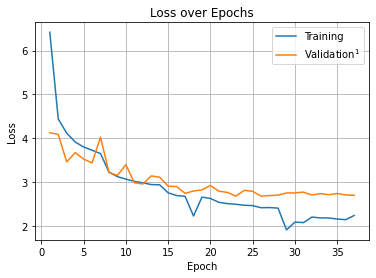
\includegraphics[scale=0.45]{flair_loss.png}
    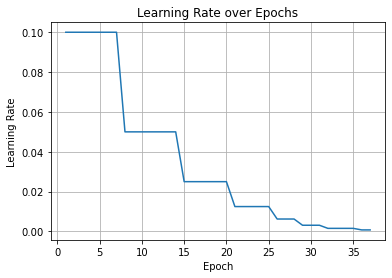
\includegraphics[scale=0.45]{flair_lrs.png}
    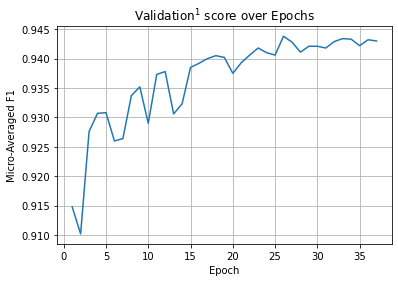
\includegraphics[scale=0.45]{flair_scores.png}
    \caption{Losses (up-left), learning rate (up-right) and Dev scores (bottom) per epoch}
    \label{fig:flairtrain}
\end{figure}
\newpage
\section{BERT$^{NER}$}
\label{sec:app:bertner}
The tables below show the results of the models for each hyperparameter configuration on Validation dataset. Table \ref{tab:bert_ner_no_scheduler} displays the results where the model was trained for 10 epochs and saved at the end of each. The Validation results are obtained on specific epochs: 2, 3, 4, 6 and 10. 2, 3 and 4 are included as they were among the recommended hyperparameters. Epoch 6 and 10 are included as the former resulted in the highest Dev ORG-F1 score while the latter was the last epoch. Table \ref{tab:bert_ner_scheduler} shows the results on Validation dataset for the setting where a linear learning rate scheduler is used.

\begin{table}[h!]
    \centering
    \begin{tabular}{c| c c c| c c c}
    &\multicolumn{3}{c|}{Organization}&\multicolumn{3}{c}{Grant} \\
    Epoch&Precision&Recall&F1&Precision&Recall&F1\\
    \hline
    2     & 80.38	&84.14&82.22	&94.18&	96.95&95.55  \\
    3     & 78.76	&84.9&81.72	&94.51&	96.78&95.63  \\
    4     & 79.18	&84.18&81.6	&94.3&	96.89&95.58  \\
    6     & 79.88	&84.71&82.23	&94.73	&96.53&95.62  \\
    10   &  81.04	&80.24&80.64	&94.62&	96.38&95.49  \\
    \end{tabular}
    \caption{BERT$^{NER}$ results on Validation. Trained for 10 epochs without a scheduler, the model is saved after every epoch.}
    \label{tab:bert_ner_no_scheduler}
\end{table}


\begin{table}[h!]
    \centering
    \begin{tabular}{c| c c c| c c c}
    &\multicolumn{3}{c|}{Organization}&\multicolumn{3}{c}{Grant} \\
    Epoch&Precision&Recall&F1&Precision&Recall&F1\\
    \hline
    2     & 78.44&	85.8&	81.96&	94.59&	97.43&	95.99
 \\
    3     & 79.18&86.03&82.46&94.71&97.39&96.03
 \\
    4     & 79.41&85.88&82.52&94.95&97.38&96.15
 \\
    \end{tabular}
    \caption{BERT$^{NER}$ results on Validation. Trained for 2,3 and 4 epochs respectively with a scheduler, the model is saved after the training is done.}
    \label{tab:bert_ner_scheduler}
\end{table}

As the scores for Grant mentions are high in each setup, the model is chosen based on the scores on Organization mentions. Recall is favored over precision and based on this intuition, the model that is trained for 3 epochs with a learning rate scheduler is selected. This model has the highest recall for Organization mentions and the second highest F1 score. 

\section{BI$_{AD}$}
\label{sec:app:biencoderadapt}
Table \ref{tab:biencoderadaptresapp} the scores of the models after each round on Training and Dev splits for BI$_{AD}$ with the second hyperparameter setting, the one where one round corresponds to two epochs and maximum number of tokens is set to 256 for the candidate representation.
\newpage
\vspace*{-3cm}\begin{table}[H]
    \centering
   \begin{tabular}{ccccc}
    &&&Micro Averaged & Macro Averaged\\
    Dataset & Round & Threshold     & Accuracy &Accuracy\\
    \hline
    Training & 1 & 0.5 & 62.36&64.44\\
    Training & 2 & 0.5 & 87.06&88.33\\
    Training & 3 & 0.5 & 90.3&91.09\\
    Training & 4 & 0.5 & 94.94&95.61\\
    \hline
    Training & 1 & 0.972&70.53&71.4 \\
    Training & 2 & 0.75 &91.66&92.29\\
    Training & 3 & 0.759&93.62&94.12 \\
    Training & 4 & 0.728&96.16&96.67 \\
    \hline
    Dev & 1 & 0.5&63.62&70.03 \\
    Dev & 2 & 0.5&82.56&87.07 \\
    Dev & 3 & 0.5&84.16&88.21 \\
    Dev & 4 & 0.5&86.26&89 \\
    \hline
    Dev & 1 & 0.972&70.24&75.05\\
    Dev & 2 & 0.75 &86.38&89.45\\
    Dev & 3 & 0.759&86.74&89.94\\
    Dev & 4 & 0.728&87.74&90.14\\
    \end{tabular}
    
    \vspace{0.5cm}\begin{tabular}{cccccc}
    &&&&EE Setting & \\
    Dataset & Round    & Threshold & Precision & Recall & F1 Score \\
    \hline
    Training & 1 & 0.5&100&0.02&0.04 \\
    Training & 2 & 0.5&96.68&57.56&72.16 \\
    Training & 3 & 0.5&99.13&67.77&80.5 \\
    Training & 4 & 0.5&99.16&87.66&93.06 \\
    \hline
    Training & 1 & 0.972&72.15&57.81&64.19 \\
    Training & 2 & 0.75&86.11&89.88&87.96 \\
    Training & 3 & 0.759&91.59&90.96&91.27 \\
    Training & 4 & 0.728 &95.85&96.45&96.15\\
    \hline 
    Dev & 1 & 0.5&0&0&0 \\
    Dev & 2 & 0.5&83.75&42.69&56.55 \\
    Dev & 3 & 0.5&87.22&44.76&59.16 \\
    Dev & 4 & 0.5&83.84&60.3&70.15 \\
    \hline
    Dev & 1 & 0.972 &66.03&55.7&60.43\\
    Dev & 2 & 0.75  &69.64&79.98&74.45\\
    Dev & 3 & 0.759 &72.9&73.99&73.44\\
    Dev & 4 & 0.728 &74.81&77.91&76.33\\
    \end{tabular}
    
    \vspace{0.5cm}\begin{tabular}{cccccc}
    &&&&InKB Setting & \\
    Dataset & Round    & Threshold& Precision & Recall & F1 Score \\
        \hline
    Training & 1 & 0.5&62.36&76.58&68.74 \\
    Training & 2 & 0.5&85.86&93.79&89.65 \\
    Training & 3 & 0.5&89.02&95.44&92.12 \\
    Training & 4 & 0.5&94.11&96.6&95.34 \\
    \hline
    Training & 1 & 0.972&70.25&73.44&71.81 \\
    Training & 2 & 0.75 &93&92.07&92.53\\
    Training & 3 & 0.759&94.08&94.23&94.16 \\
    Training & 4 & 0.728&96.23&96.09&96.16 \\
    \hline
    Dev & 1 & 0.5&63.62&75.26&68.95\\
    Dev & 2 & 0.5&82.45&89.85&85.99\\
    Dev & 3 & 0.5&83.89&91.37&87.47\\
    Dev & 4 & 0.5&86.56&91.01&88.73\\
    \hline
    Dev & 1 & 0.972&70.87&72.9&71.87 \\
    Dev & 2 & 0.75 &90&87.56&88.76 \\
    Dev & 3 & 0.759&89.32&89.07&89.2 \\
    Dev & 4 & 0.728&90.22&89.53&89.87 \\
    \end{tabular}
    \caption{Intermediate Results for BI$_{AD}$}
    \label{tab:biencoderadaptresapp}
\end{table}

\end{document}

